\newpage
\chapter{TINJAUAN PUSTAKA} \label{Bab II}

\section{Tinjauan Pustaka} \label{II.Tinjauan}
Tinjauan pustaka berisi berbagai penelitian terdahulu yang memiliki kesamaan topik dengan penelitian ini dan digunakan sebagai referensi utama. Penelitian ini merujuk pada beberapa studi literatur yang membahas metode serta pendekatan yang akan diterapkan. Berikut adalah beberapa penelitian yang di jadikan acuan.\par

Penelitian yang dilakukan oleh N. Aditama dan R. Munir pada tahun 2022 mengusulkan metode estimasi kalori makanan jalanan Indonesia menggunakan \textit{Mask} R-CNN untuk segmentasi makanan dan \textit{Multiple Linear Regression} (MLR) untuk estimasi kalori yang menerapkan teknik \textit{amodal instance segmentation} menggunakan beberapa \textit{backbone} seperti ResNet-101-FPN dan ResNetXt-101-FPN. Dataset terdiri dari 1.646 citra makanan dengan enam kelas mencakup 4.530 total objek menggunakan optimizer \textit{Stochastic Gradient Descent} (SGD). Hasil pengujian terbaik diperoleh menggunakan \textit{Mask} R-CNN ResNeXt-101-FPN dengan nilai \textit{F1-Score} sebesar 0,821 pada kondisi tertutup dengan \textit{F1-Score} sebesar 0,994 pada kondisi tidak tertutup, dan rata-rata R² = 0,80425 pada model regresi \cite{FoodMaskRCNN10}. \par

Penelitian yang dilakukan oleh K. Tang, \textit{et.al} pada tahun 2025 yang mengembangkan \textit{Improved Mask} R-CNN dengan menambahkan  \textit{Re-parameterized Refocus Convolution} (RefConv) dan \textit{Efficient Channel Attention} (ECA). Dataset yang digunakan berjumlah 3,500 gambar yang dilatih selama 100 epoch. Hasil eksperimen berhasil meningkatkan ketelitian segmentasi pada citra bijih yang mencapai MIoU 92,8\% dan mAP 97,2\% yang lebih tinggi daripada Mask R-CNN standar MIoU 85,88\% dan mAP 92,10\% menunjukkan bahwa kombinasi RefConv dan ECA berhasil meningkatkan kemampuan model dalam meningkatkan akurasi segmentasi \cite{OreSegmentation2}. \par

Penelitian yang dilakukan oleh H. Zhou, G. Cai, dan S. Liu pada tahun 2023 mengusulkan \textit{Improved Mask} R-CNN untuk mendeteksi bijih yang bertumpuk menggunakan arsitektur ResNet-101 dengan modifikasi \textit{Multipath Feature Pyramid Network} (MFPN) yang memperkaya detail fitur dari citra bijih. Dataset yang digunakan berjumlah 1,000 gambar yang dilatih selama 200 epoch menggunakan \textit{optimizer Adam}. Hasil eksperimen menunjukkan peningkatan kinerja dengan nilai $AP_{75}$ dengan jaringan fusi fitur yang ditingkatkan mencapai sekitar 73,12\%, sekitar 6,64\% lebih tinggi dibanding \textit{Mask} R-CNN standar \cite{ImprovedMaskRCNNOrePanggangan}. \par

Penelitian yang dilakukan oleh B.A.P. Ferreira, \textit{et.al} pada tahun 2024 mengusulkan penerapan \textit{Mask} R-CNN untuk mengidentifikasi dan melakukan segmentasi partikel kuarsa pada citra mikroskop bijih besi menggunakan pendekatan \textit{instance segmentation}. Dataset terdiri dari 865 citra yang berisi 1.740 partikel kuarsa yang dilabel secara manual menggunakan perangkat VGG \textit{Image Annotator} (VIA) dengan menggunakan \textit{backbone} ResNet-101 dengan optimasi menggunakan \textit{stochastic gradient descent}. Hasil pengujian menunjukkan performa yang sangat baik dengan \textit{precision} sebesar 95,22\%, \textit{recall} 88,46\%, dan \textit{F1-score} 91,72\% yang menunjukkan kemampuan tinggi model dalam mengenali dan memisahkan partikel kuarsa dari latar belakang kompleks \cite{QuartzMicMaskrcnn}. \par

Penelitian yang dilakukan oleh M.R. Iyas, N.I. Setiawan, dan I.W. Warmada pada tahun 2020 mengusulkan penggunaan \textit{Mask} R-CNN untuk identifikasi mineral pembentuk batuan pada citra \textit{petrography} menggunakan empat model berbeda berdasarkan pencahayaan mikroskop \textit{Plane Polarized Light} (PPL) dan \textit{Cross Polarized Light} (XPL) serta jenis \textit{backbone} (ResNet-50 dan ResNet-101). Hasil pengujian menunjukkan bahwa model terbaik adalah Model B (ResNet-101 + pencahayaan) dengan AP 58,0\% sebagai yang terbaik, mengungguli Model A (57,8\%), Model C (45,8\%), dan Model D (43,6\%), serta bahwa pencahayaan mikroskop meningkatkan performa sekitar 12–14,4\% \cite{maskrcnnKalimantanMic}. \par
 
Penelitian yang dilakukan oleh E.J.Y. Koh, \textit{et.al} pada tahun 2021 melakukan penelitian mengenai otomatisasi analisis mineralogi menggunakan dua algoritma segmentasi berbasis \textit{deep learning}, yaitu \textit{Mask} R-CNN dan SOLO v2. Dataset terdiri atas 122 citra mikroskop dengan tiga kelas utama. Model Mask R-CNN dilatih selama 303 epoch dengan hasil $AP_{coco}$ sebesar 44,3\% dengan 5 frame/detik, sementara SOLO v2 di latih selama 45 epoch menghasilkan $AP_{coco}$ sebesar 50,4\% dengan 20 frame/detik yang menunjukan bahwa model \textit{instance segmentation} mampu mendeteksi mineral secara cepat dan akurat \cite{mineralogiMaskRCNNSolo}. Berikut pada Tabel \ref{table:2.Tinjauan} dilampirkan ringkasan tinjauan pustaka terdahulu. \par

% Penelitian yang dilakukan oleh L. Qi, \textit{et.al} mengusulkan metode \textit{amodal instance segmentation} melalui pengenalan dataset baru, KINS (KITTI INStance dataset). Mereka mengusulkan arsitektur \textit{Amodal Segmentation Network} (ASN) untuk memprediksi bentuk utuh objek termasuk bagian yang tidak terlihat atau teroklusi, yang menerapkan teknik \textit{Multi-Level Coding} (MLC) dan sebuah \textit{Occlusion Classification Branch}. Metode ini diimplementasikan di atas \textit{baseline} \textit{state-of-the-art} seperti \textit{Mask} R-CNN. Dataset KINS terdiri dari 14.991 total citra, dibagi menjadi 7.474 citra latih dan 7.518 citra uji, dengan anotasi padat untuk 7 kategori objek. Model dilatih menggunakan optimizer \textit{Stochastic Gradient Descent} (SGD). Hasil pengujian menunjukkan ASN meningkatkan kinerja \textit{baseline} secara signifikan, di mana \textit{Mask} R-CNN + ASN menghasilkan rata-rata presisi (\textit{mAP}) sebesar 32{,}7\% untuk deteksi (dibanding 31{,}3\%), 31{,}1\% untuk \textit{amodal segmentation} (dibanding 29{,}3\%), dan 28{,}7\% untuk \textit{inmodal segmentation} (dibanding 26{,}6\%) \cite{AmodalASN}. Berikut pada Tabel \ref{table:2.Tinjauan} dilampirkan ringkasan tinjauan pustaka terdahulu.\par

% Atur margin untuk landscape - bisa disesuaikan nilai left dan right
\newgeometry{top=2cm, bottom=1.75cm, left=2.25cm, right=2cm}
\begin{landscape}
% \thispagestyle{landscape} % Untuk page number yang benar di landscape
\begin{longtable}{|p{0.2cm}|p{1.6cm}|p{2.4cm}|p{2.5cm}|p{2.5cm}|p{2.5cm}|p{3.5cm}|}
	\caption{Penelitian Terdahulu}
	\label{table:2.Tinjauan}\\
	\hline
	\multicolumn{1}{|c|}{\textbf{No.}} & 
	\multicolumn{1}{c|}{\textbf{Peneliti}} & 
	\multicolumn{1}{c|}{\textbf{Judul}} & 
	\multicolumn{1}{c|}{\textbf{Metode Seleksi Fitur}} & 
	\multicolumn{1}{c|}{\textbf{Permasalahan}} & 
	\multicolumn{1}{c|}{\textbf{Metode Klasifikasi}} &
	\multicolumn{1}{c|}{\textbf{Hasil}} \\
	\hline
	\endfirsthead
	
	% \multicolumn{7}{c}{\tablename\ \thetable\ -- \textit{Lanjutan dari halaman sebelumnya}} \\
	\hline
	\multicolumn{1}{|c|}{\textbf{No.}} & 
	\multicolumn{1}{c|}{\textbf{Peneliti}} & 
	\multicolumn{1}{c|}{\textbf{Judul}} & 
	\multicolumn{1}{c|}{\textbf{Metode Seleksi Fitur}} & 
	\multicolumn{1}{c|}{\textbf{Permasalahan}} & 
	\multicolumn{1}{c|}{\textbf{Metode Klasifikasi}} &
	\multicolumn{1}{c|}{\textbf{Hasil}} \\
	\hline
	\endhead
	
	\hline
	% \multicolumn{7}{r}{\textit{Bersambung ke halaman berikutnya}} \\
	\endfoot
	
	\hline
	\endlastfoot
	
	1. & 
	N. Aditama, dan R. Munir (2022) \cite{FoodMaskRCNN10}& 
	\textit{Indonesian Street Food Calorie Estimation using Mask R-CNN and Multiple Linear Regression} & 
	ResNet-101-FPN, ResNeXt-101-FPN, \textit{Amodal instance segmentation} & 
	Segmentasi pada citra makanan dengan objek yang saling menutupi \textit{(occlusion)} serta variasi bentuk yang kompleks & 
	\textit{Mask} R-CNN, \textit{Multiple Linear Regression} & 
	Model ResNeXt-101-FPN mencapai \textit{F1-score} 0,821 pada kondisi tertutup, 0,994 pada kondisi tidak tertutup, dan R² 0,80425 untuk regresi kalori \\
	\hline
	
	2. & 
	K. Tang, \textit{et al.} (2025) \cite{OreSegmentation2}& 
	\textit{Improvement of Mask R-CNN Algorithm for Ore Segmentation} & 
	\textit{Re-parameterized Refocus Convolution} (RefConv), \textit{Efficient Channel Attention} (ECA), ResNet-50  & 
	Segmentasi bijih \textit{polymetallic nodules} kurang akurat pada model standar akibat hilangnya detail tepi & 
	\textit{Improvement Mask} R-CNN & 
	Model \textit{Improvement Mask} R-CNN menghasilkan MIoU 92,8\% dan mAP 97,2\% yang meningkat signifikan dari model standar dengan MIoU 85,88\% dan mAP 92,10\% \\
	\hline
	 
	3. & 
	H. Zhou, G. Cai, dan S. Liu (2023) \cite{ImprovedMaskRCNNOrePanggangan}& 
	\textit{Research on stacked ore detection based on improved Mask RCNN under complex background} & 
	\textit{Multipath Feature Pyramid Network} (MFPN) dengan ResNet-101 & 
	Deteksi bijih yang saling bertumpuk pada latar belakang kompleks & 
	\textit{Improvement Mask} R-CNN & 
	Model dengan MFPN mencapai $AP_{75}$ sebesar 73,12\%, meningkat 6,64\% dibanding \textit{Mask} R-CNN standar \\
	\hline

	4. & 
	B.A.P. Ferreira \textit{et al.} (2024) \cite{QuartzMicMaskrcnn} & 
	\textit{Instance Segmentation of Quartz in Iron Ore Optical Microscopy Images by Deep Learning} & 
	ResNet-101, VGG \textit{Image Annotator} (VIA) & 
	Segmentasi partikel kuarsa yang memiliki sifat transparan dan warna serupa dengan resin pengikat & 
	\textit{Mask} R-CNN & 
	Model \textit{Mask} R-CNN mencapai \textit{precision} sebesar 95,22\%, \textit{recall} 88,46\%, dan \textit{F1-score} 91,72\% dalam segmentasi partikel kuarsa \\
	\hline

	5. & 
	M.R. Iyas, N.I. Setiawan, dan I.W. Warmada (2020) \cite{maskrcnnKalimantanMic}& 
	\textit{Mask R-CNN for rock-forming minerals identification on petrography, case study at Monterado, West Kalimantan} & 
	ResNet-50, ResNet-101, \textit{Plane Polarized Light} (PPL), \textit{Cross Polarized Light} (XPL) & 
	Identifikasi mineral pembentuk batuan pada citra yang dipengaruhi oleh perbedaan pencahayaan mikroskop & 
	\textit{Mask} R-CNN & 
	Model terbaik adalah model B (ResNet-101 dengan pencahayaan) memperoleh AP 58,0\% yang lebih tinggi 12-14\% dibanding model tanpa pencahayaan \\
	\hline

	6. & 
	E.J.Y. Koh \textit{et al.} (2021) \cite{mineralogiMaskRCNNSolo}& 
	\textit{Utilising convolutional neural networks to perform fast automated modal mineralogy analysis for thin-section optical microscopy} & 
	ResNet, SOLO v2, \textit{Feature Pyramid Network} (FPN) & 
	Segmentasi mineral untuk analisis mineralogi modal otomatis pada mikroskop optik \textit{thin-section} & 
	\textit{Mask} R-CNN, SOLO v2 & 
	\textit{Mask} R-CNN menghasilkan $AP_{coco}$ 44,3\% dengan kecepatan 5 frame/ detik, sedangkan SOLO v2 mencapai $AP_{coco}$ 50,4\% dengan kecepatan 20 frame/detik. \\
	\hline

	
	% 7. & 
	% L. Qi \textit{et al.}  & 
	% \textit{Amodal Instance Segmentation with KINS Dataset} (2019) \cite{AmodalASN} & 
	% \textit{Amodal Segmentation Network} (ASN), \textit{Multi-Level Coding} (MLC), Occlusion \textit{Classification Branch} & 
	% Model standar gagal memprediksi bagian objek yang teroklusi \textit{(amodal)} karena \textit{overfitting} pada fitur lokal yang terlihat. & 
	% Mask R-CNN, PANet & 
	% Metode ASN (dengan MLC) meningkatkan mAP sebesar 32{,}7\% untuk deteksi (dibanding 31{,}3\%), 31{,}1\% untuk \textit{amodal segmentation} (dibanding 29{,}3\%), dan 28{,}7\% untuk \textit{inmodal segmentation} (dibanding 26{,}6\%). \\ 
	% \hline
	
\end{longtable}
\end{landscape}
\restoregeometry
% \pagestyle{fancy} % Kembalikan ke pagestyle normal setelah landscape

Berdasarkan informasi yang telah disajikan pada Tabel 2.1, terdapat sejumlah perbedaan dan pembaruan dibandingkan dengan penelitian terdahulu. Penelitian ini berfokus pada identifikasi mineral kasiterit dari citra mikroskop menggunakan model \textit{Mask} R-CNN dengan penerapan teknik \textit{amodal instance segmentation} untuk mengatasi oklusi antarbutir mineral. Evaluasi performa dilakukan menggunakan metrik AP dan IoU guna menilai ketepatan deteksi dan akurasi segmentasi \par

\section{Dasar Teori} \label{II.Teori}
Dasar teori merupakan landasan intelektual yang memberikan pemahaman menyeluruh terhadap konsep-konsep yang relevan dengan penelitian, menjelaskan prinsip-prinsip teoretis yang mendasari kajian, serta membentuk kerangka konseptual yang menjadi acuan dalam pengembangan metode, analisis, dan interpretasi hasil penelitian secara ilmiah dan terarah. \par

\subsection{Kasiterit} \label{II.TeoriKasiterit}
Kasiterit (\senyawatin) dikenal juga dengan nama \textit{Tinstone} merupakan mineral utama pembentuk timah yang secara teoritis mengandung 78\% timah, namun karena jarang ditemukan dalam bentuk murni, maka kandungan timahnya hanya sekitar 73–75\% \cite{PurificationCassiterite4} \cite{bookTin}. Mineral ini memiliki struktur kristal tetragonal yang memiliki sifat \textit{opaque} yang dapat tembus pada sayatan tipis dan kilap \textit{adamantin} hingga \textit{submetallic}. Kasiterit memiliki densitas tinggi (sekitar $7,15~g/cm^3$) yang sangat tahan terhadap pelapukan dan di klasifikasikan sebagai mineral berat \cite{GeochemicalGeologicalTin}. Mineral kasiterit yang di ambil pada citra mikroskop dapat di lihat pada Gambar \ref{fig:2.Kasiterit} berikut. \par

\begin{figure}[H] % Kalau menggunakan H, posisi gambar akan tepat dibawah teks
    \centering
    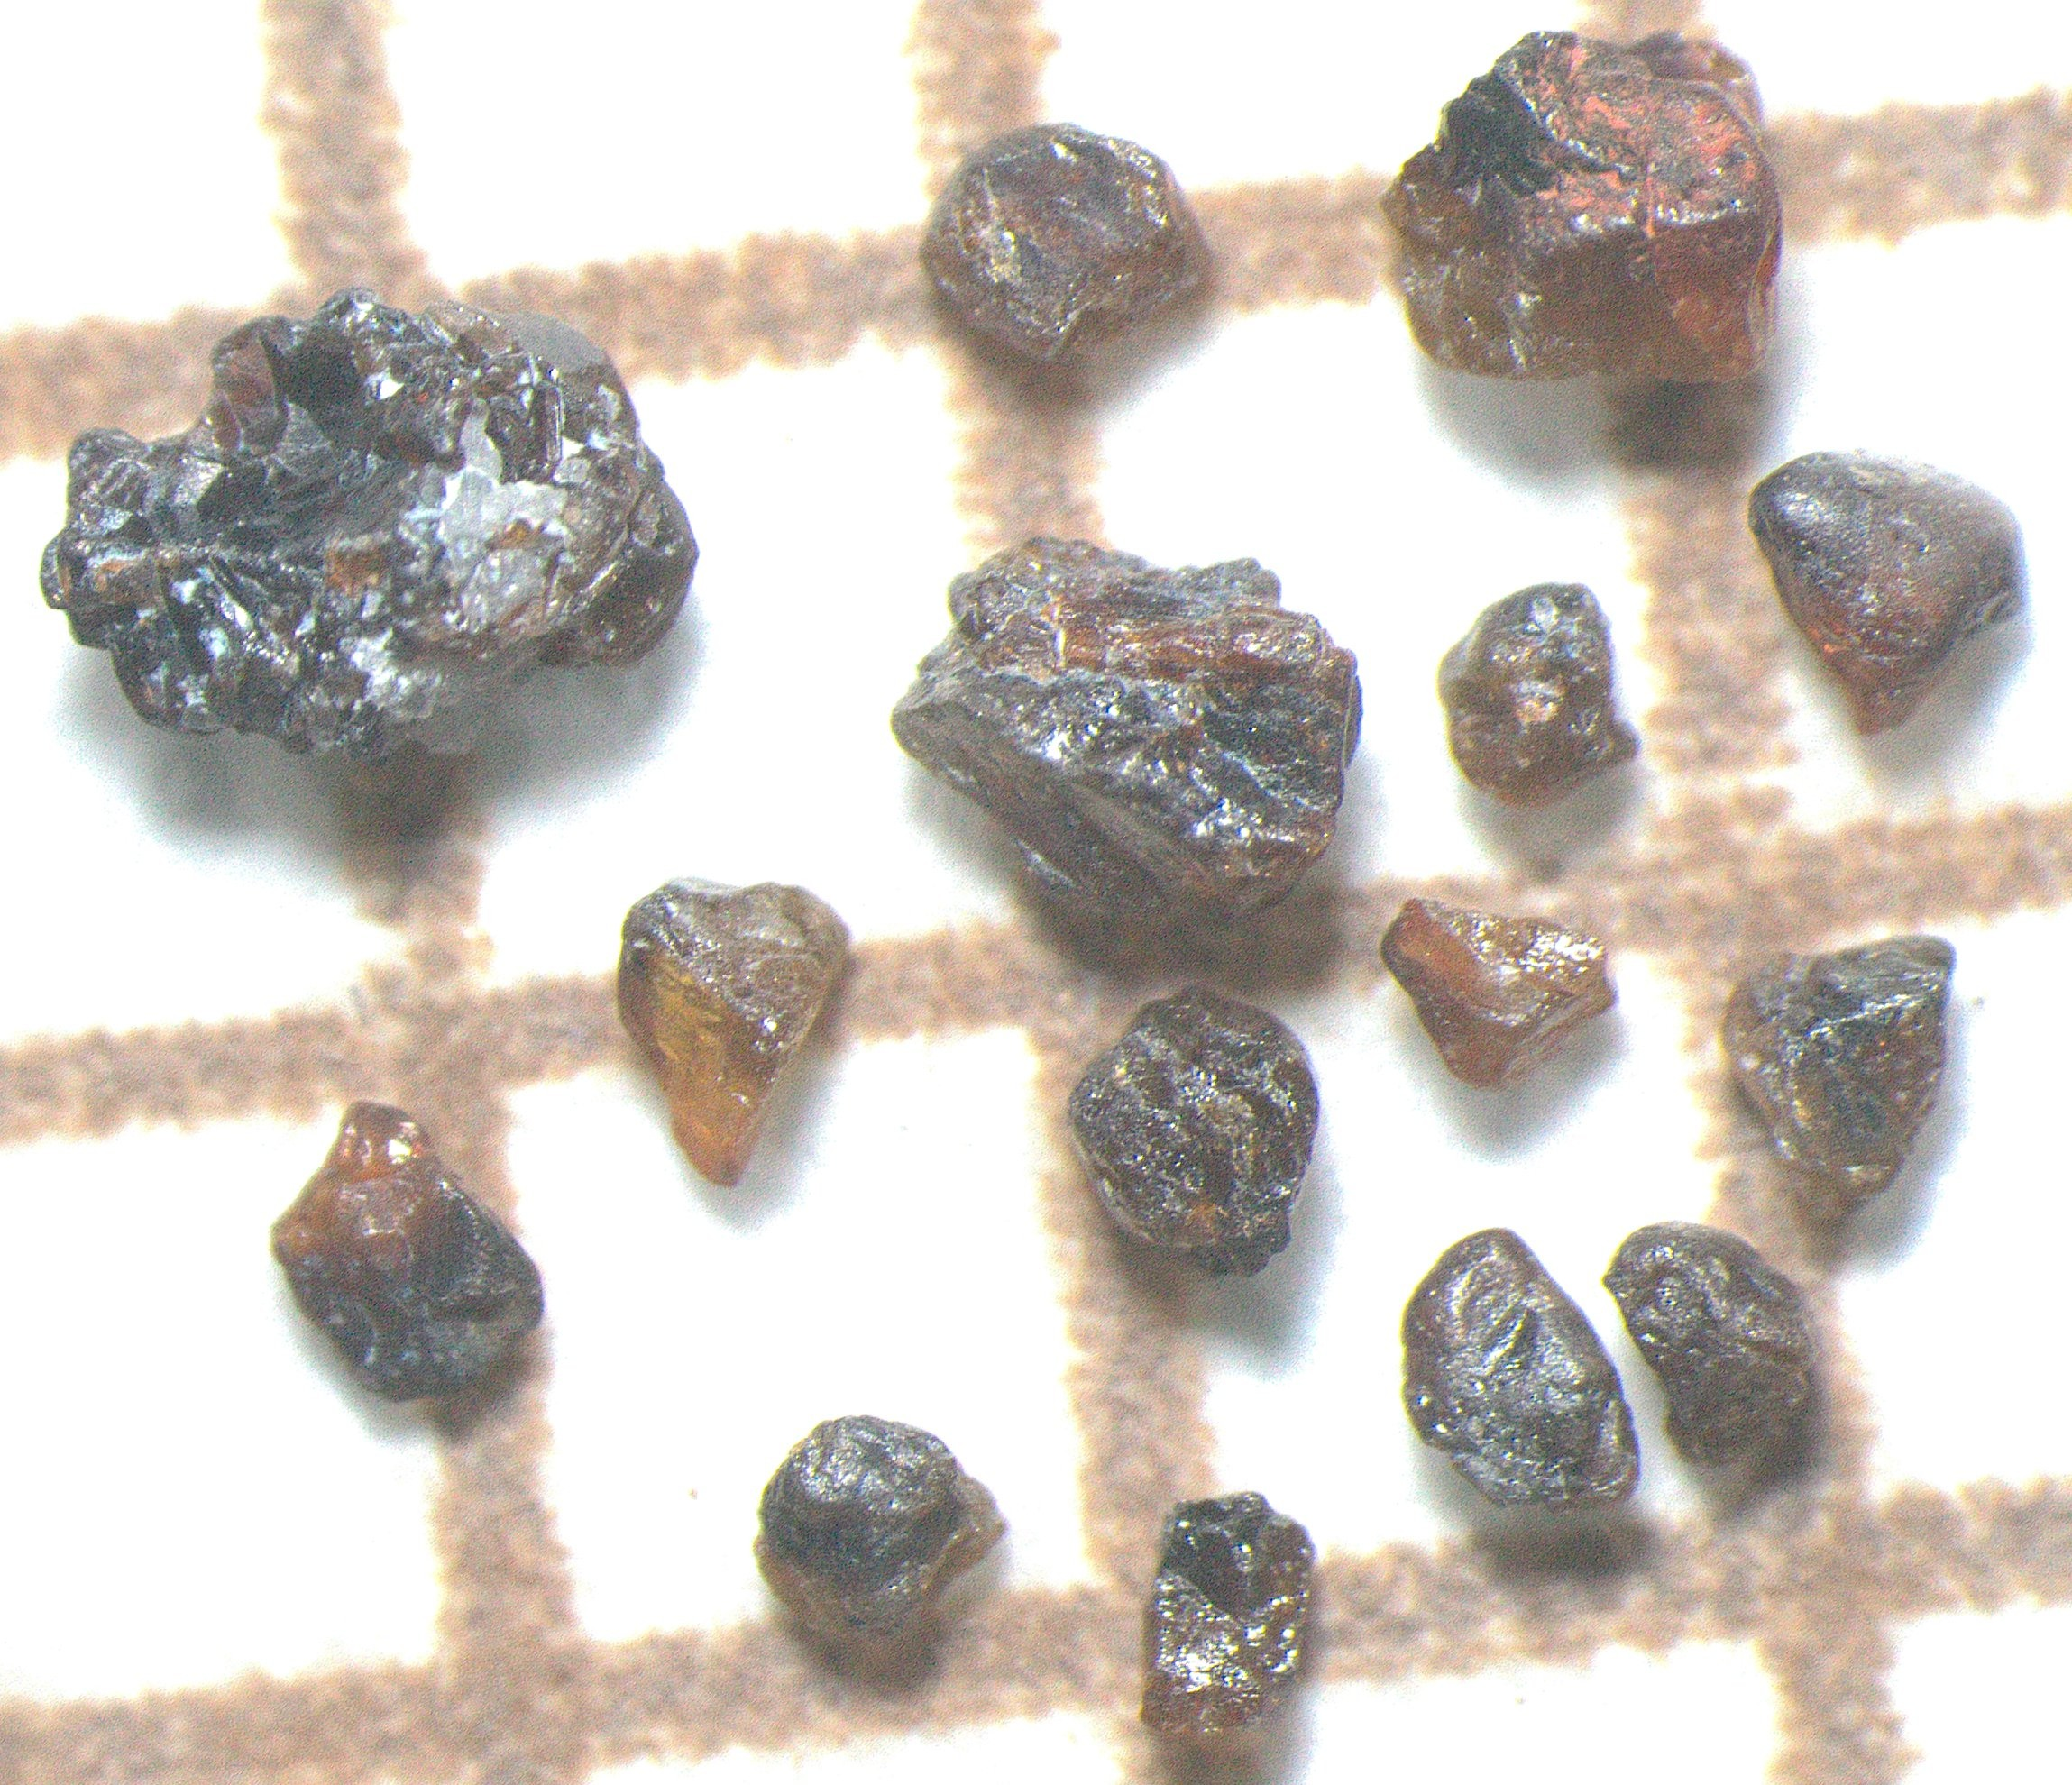
\includegraphics[width=0.5\textwidth]{figure/cassiteriteImg.jpg}
    \caption{Mineral Kasiterit}
    \label{fig:2.Kasiterit}
\end{figure}

Mineral kasiterit umumnya berwarna coklat gelap hingga hitam, meskipun variasi kemerahan atau kekuningan dapat terjadi karena pengotor utama seperti tantalum, niobium, titanium, dan unsur-unsur lainnya dalam bentuk \textit{solid solution} \cite{IrzonTimahIndonesia12} \cite{bookTin}. Setidaknya terdapat 14 mineral pembawa timah lainnya dan sebagian di antaranya hanya ditemukan pada wilayah tertentu \cite{IrzonTimahIndonesia12}. Pada wilayah-wilayah tersebut, kasiterit umumnya hadir bersama mineral ikutan seperti ilmenit, pasir kuarsa, zirkon, rutil, pirit, kalsit, lantanum, dan monasit, yang merupakan sumber potensial unsur tanah jarang (UTJ) \cite{PurificationCassiterite4} \cite{IrzonTimahIndonesia12}. Detail karakteristik kasiterit dapat dilihat pada Tabel \ref{table:ciri2-kasiterit} berikut. \par

\begin{longtable}{|p{0.04\textwidth}|p{0.26\textwidth}|p{0.60\textwidth}|}
\caption{Ciri-ciri Kasiterit}
\label{table:ciri2-kasiterit} \\
\hline
\centering\textbf{No.} & \centering\textbf{Ciri} & \centering\arraybackslash\textbf{Spesifikasi} \\
\hline
\endfirsthead

\hline
\centering\textbf{No.} & \centering\textbf{Ciri} & \centering\arraybackslash\textbf{Spesifikasi} \\
\hline
\endhead

1 &
Warna &
Kasiterit memiliki variasi warna seperti hitam, coklat, coklat gelap, hingga merah gelap, tergantung kondisi mineral dan kandungan unsur jejaknya. \\
\hline

2 &
Kilap &
Kasiterit memiliki kilap minyak (\textit{oil luster}) yang tampak seperti permukaan berminyak saat diamati di bawah mikroskop. \\
\hline

3 &
Bentuk Butir &
Bentuk butir kasiterit umumnya membulat hingga setengah membulat (\textit{rounded} sampai \textit{sub-rounded}) dan tidak bersudut tajam. \\
\hline

4 &
Tekstur Visual &
Pada pengamatan mikroskop, kasiterit sering terlihat memiliki tekstur menyerupai daging atau serat halus. \\
\hline

5 &
Pembeda Utama &
Ciri utama pembeda kasiterit dengan mineral lain yang mirip adalah kilap minyaknya yang khas dibandingkan mineral seperti ilmenit. \\
\hline

6 &
Transparansi &
Kasiterit bersifat opak hingga tembus cahaya (translusen), terutama pada sayatan tipis atau kristal berukuran kecil. \\
\hline

7 &
Goresan (\textit{Streak}) &
Warna goresan kasiterit umumnya coklat pucat hingga putih, dan pada beberapa sampel tidak meninggalkan jejak goresan yang jelas. \\
\hline

\end{longtable}

\subsubsection{Timah} \label{II.TeoriTimah}
Timah (Sn) adalah unsur logam yang di temukan dalam bentuk mineral di alam dengan nomor atom 50 dan massa atom 118,71 \cite{IrzonTimahIndonesia12} \cite{GeochemicalGeologicalTin}. Logam ini memiliki titik lebur yang relatif rendah (232°C) dan ketahanan yang baik terhadap korosi dan oksidasi, membuatnya mudah di dilelehkan dan dilebur yang telah dimanfaatkan manusia sejak ribuan tahun lalu \cite{IrzonTimahIndonesia12}. PT. Timah Tbk. merupakan perusahaan pertambangan timah terbesar di Indonesia yang memiliki peran penting dalam kegiatan eksplorasi, penambangan, dan pengolahan bijih timah \cite{PTTimahWebsite}. Salah satu produk timah yang dihasilkan oleh PT. Timah Tbk dikenal dengan merek dagang Banka, yang merupakan bentuk timah batangan hasil proses peleburan dan pemurnian bijih timah,sebagaimana dapat dilihat pada Gambar \ref{fig:2.TimahBanka} berikut. \par

\begin{figure}[H] % Kalau menggunakan H, posisi gambar akan tepat dibawah teks
	\centering
		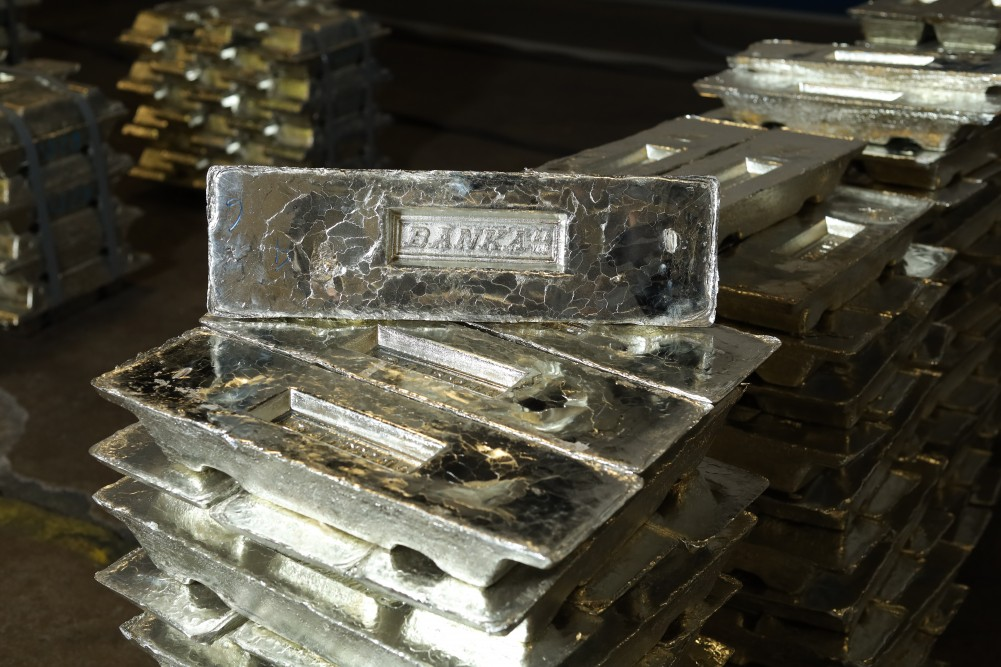
\includegraphics[width=0.5\textwidth]{figure/timahBanka.jpg}
		\caption{Produk Timah (\textit{Brand} Banka) \cite{PTTimahWebsite}}
		\label{fig:2.TimahBanka}
\end{figure}


\subsection{Citra Digital} \label{II.TeoriCitra}
Citra adalah suatu cahaya pada bidang dua dimensi. Secara matematis, citra merupakan fungsi kontinu dari intensitas cahaya pada bidang dua dimensi. Dalam konteks digital, citra adalah kumpulan titik yang dinamakan piksel (\textit{pixel} atau \textit{picture element}) \cite{bookCitra}. Setiap piksel digambarkan sebagai satu kotak kecil yang memiliki koordinat posisi. Sebuah citra digital dapat direpresentasikan sebagai ruang diskrit berdimensi-dua yang berasal dari citra analog melalui proses sampling atau digitalisasi \cite{bookCitra}. \par

\subsubsection{Citra Mikroskop} \label{II.TeoriCitraMikroskop}
Citra mikroskop pada dasarnya adalah kumpulan data intensitas foton yang berfungsi untuk memperlihatkan detail halus dalam struktur suatu objek atau sampel. Citra ini terbentuk ketika cahaya berinteraksi dengan materi yang menyusun sampel yang sedang diamati. Intensitas interaksi cahaya ini, yang menentukan kecerahan gambar, diatur secara tepat menggunakan pengatur intensitas lampu (\textit{rheostat}) \cite{microscope}. Variasi pencahayaan mikroskop berpengaruh terhadap kualitas citra yang dihasilkan, baik dari segi ketajaman maupun kontras objek mineral. Perbandingan tingkat kecerahan tersebut dapat dilihat pada Gambar \ref{fig:2.MicComparison}, yang menunjukkan perbedaan antara citra terlalu gelap, pencahayaan optimal, dan terlalu terang. \par

\begin{figure}[H]
    \centering
    % Baris pertama: dua gambar sejajar
    \begin{subfigure}[b]{0.475\textwidth}
        \centering
        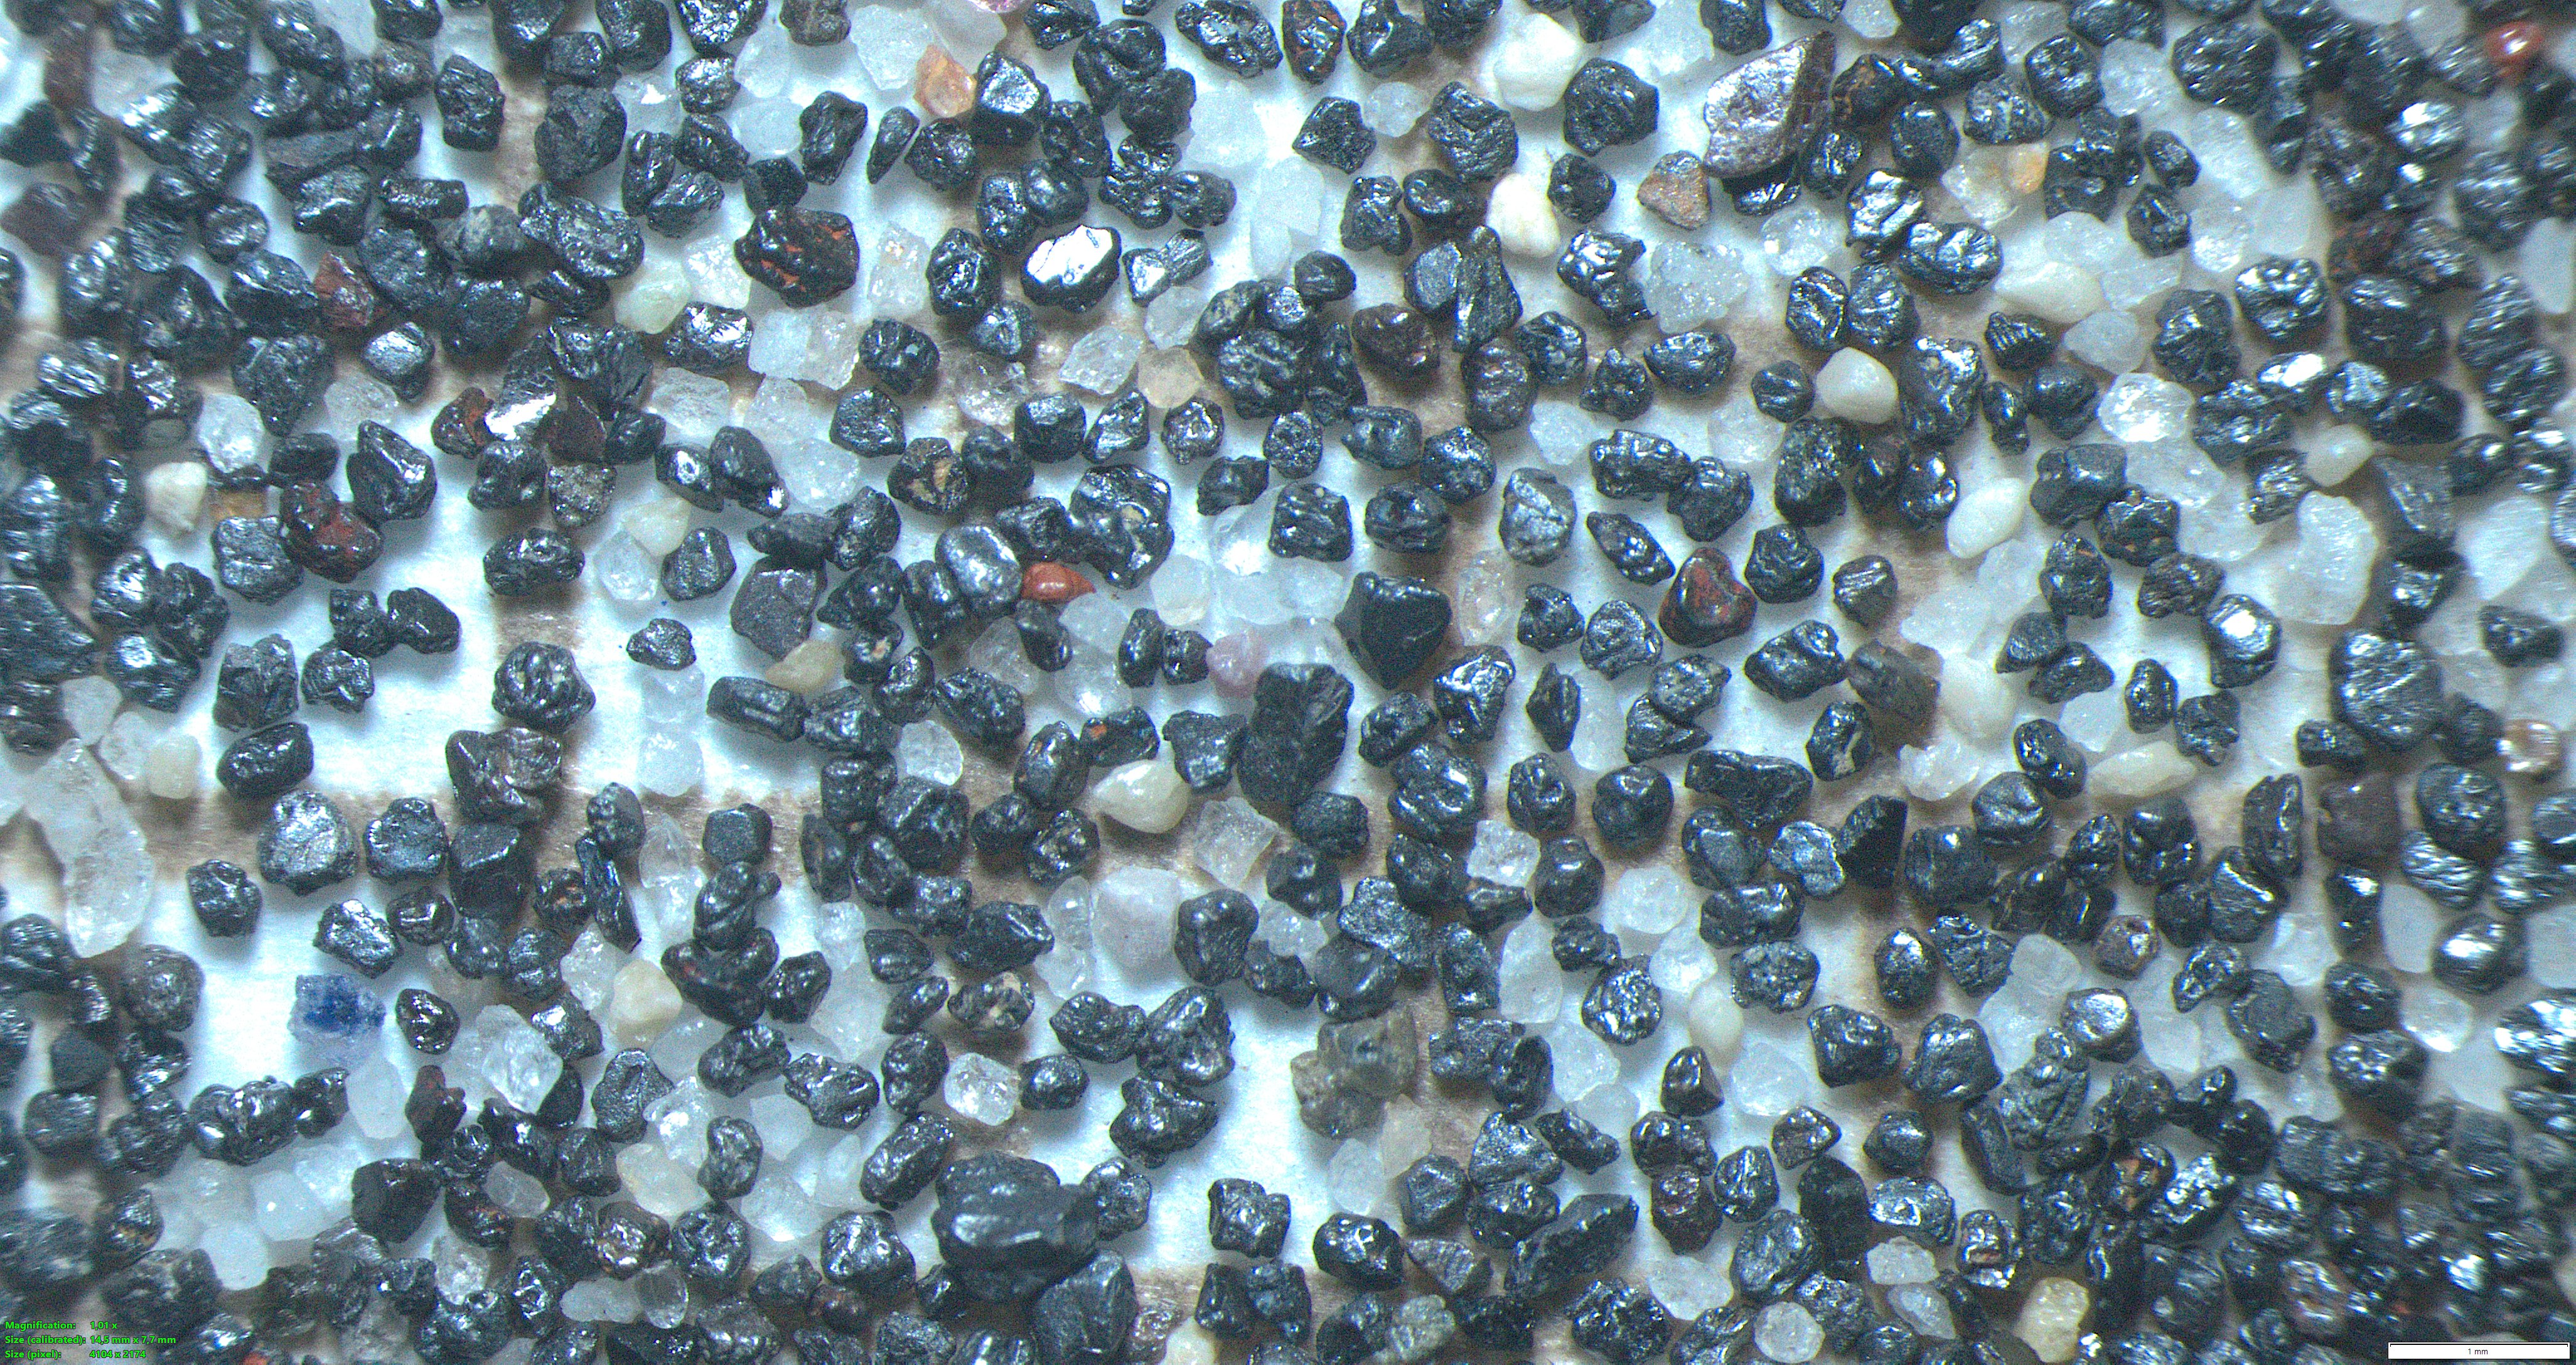
\includegraphics[width=\textwidth]{figure/micGelap.jpg}
        \caption{Kecerahan Citra Mikroskop Terlalu Gelap}
        \label{fig:2.Mic1}
    \end{subfigure}
    \hfill
    \begin{subfigure}[b]{0.475\textwidth}
        \centering
        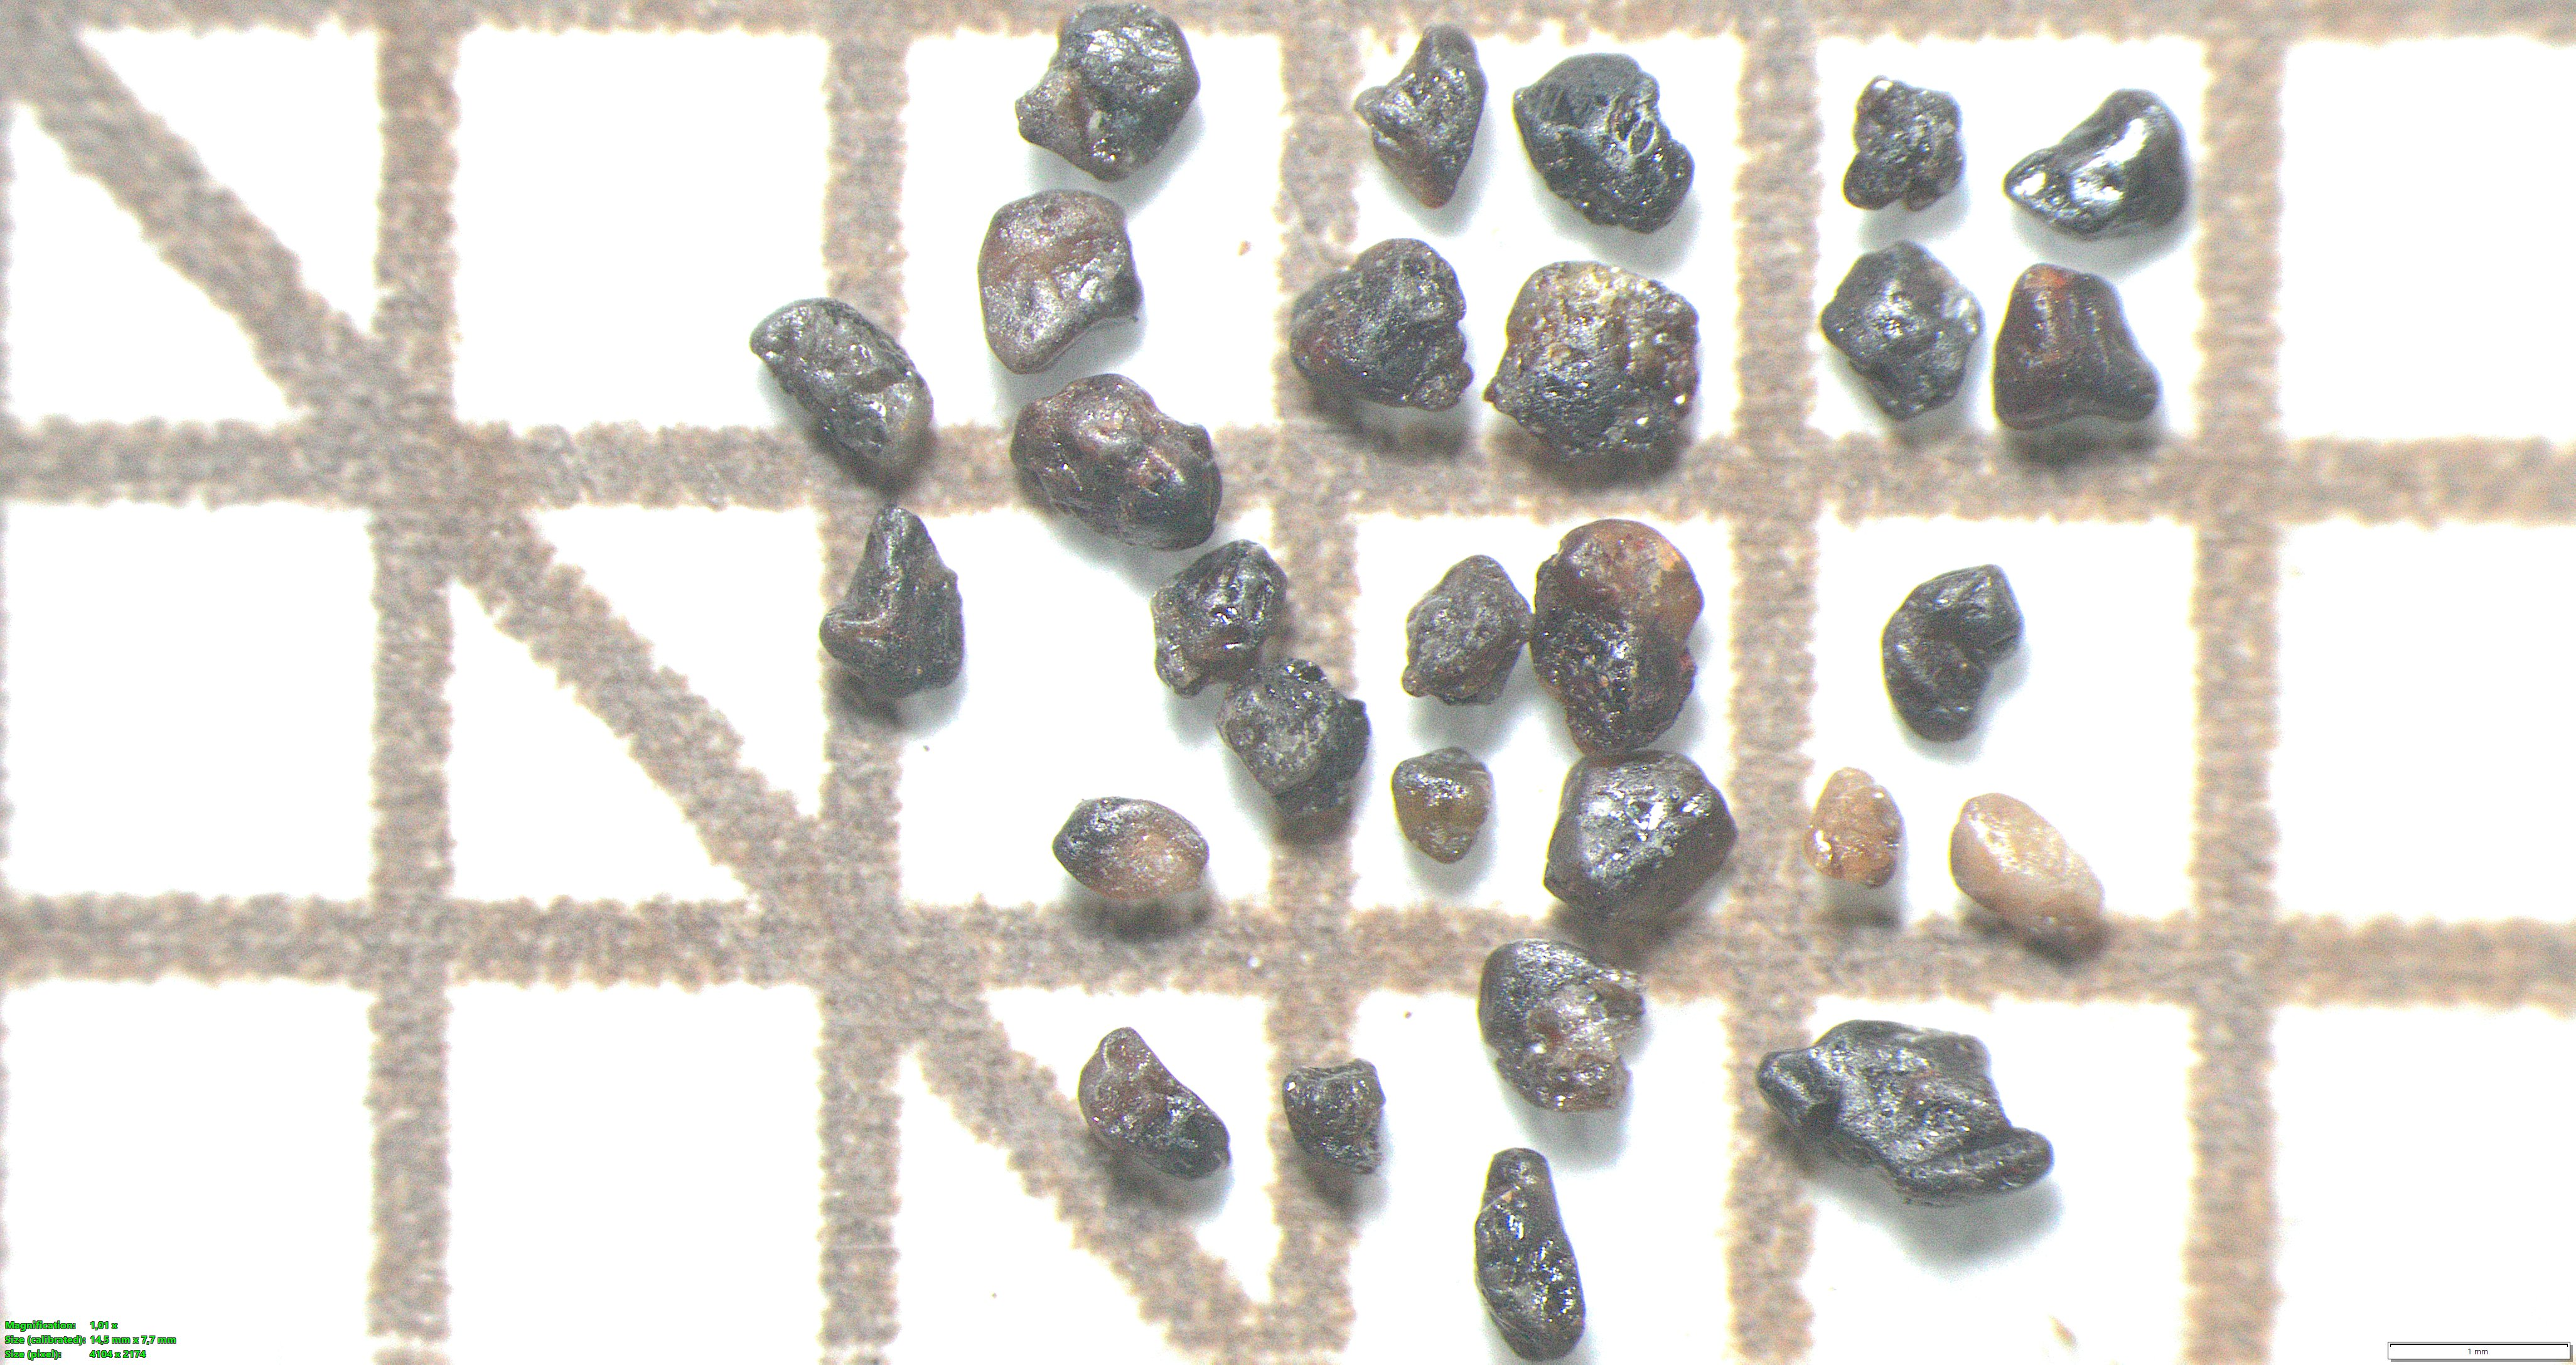
\includegraphics[width=\textwidth]{figure/micTerang.jpg}
        \caption{Kecerahan Citra Mikroskop Terlalu Terang}
        \label{fig:2.Mic3}
    \end{subfigure}
    
    % Baris kedua: satu gambar di bawah tengah
    \vskip\baselineskip
    \begin{subfigure}[b]{0.475\textwidth}
        \centering
        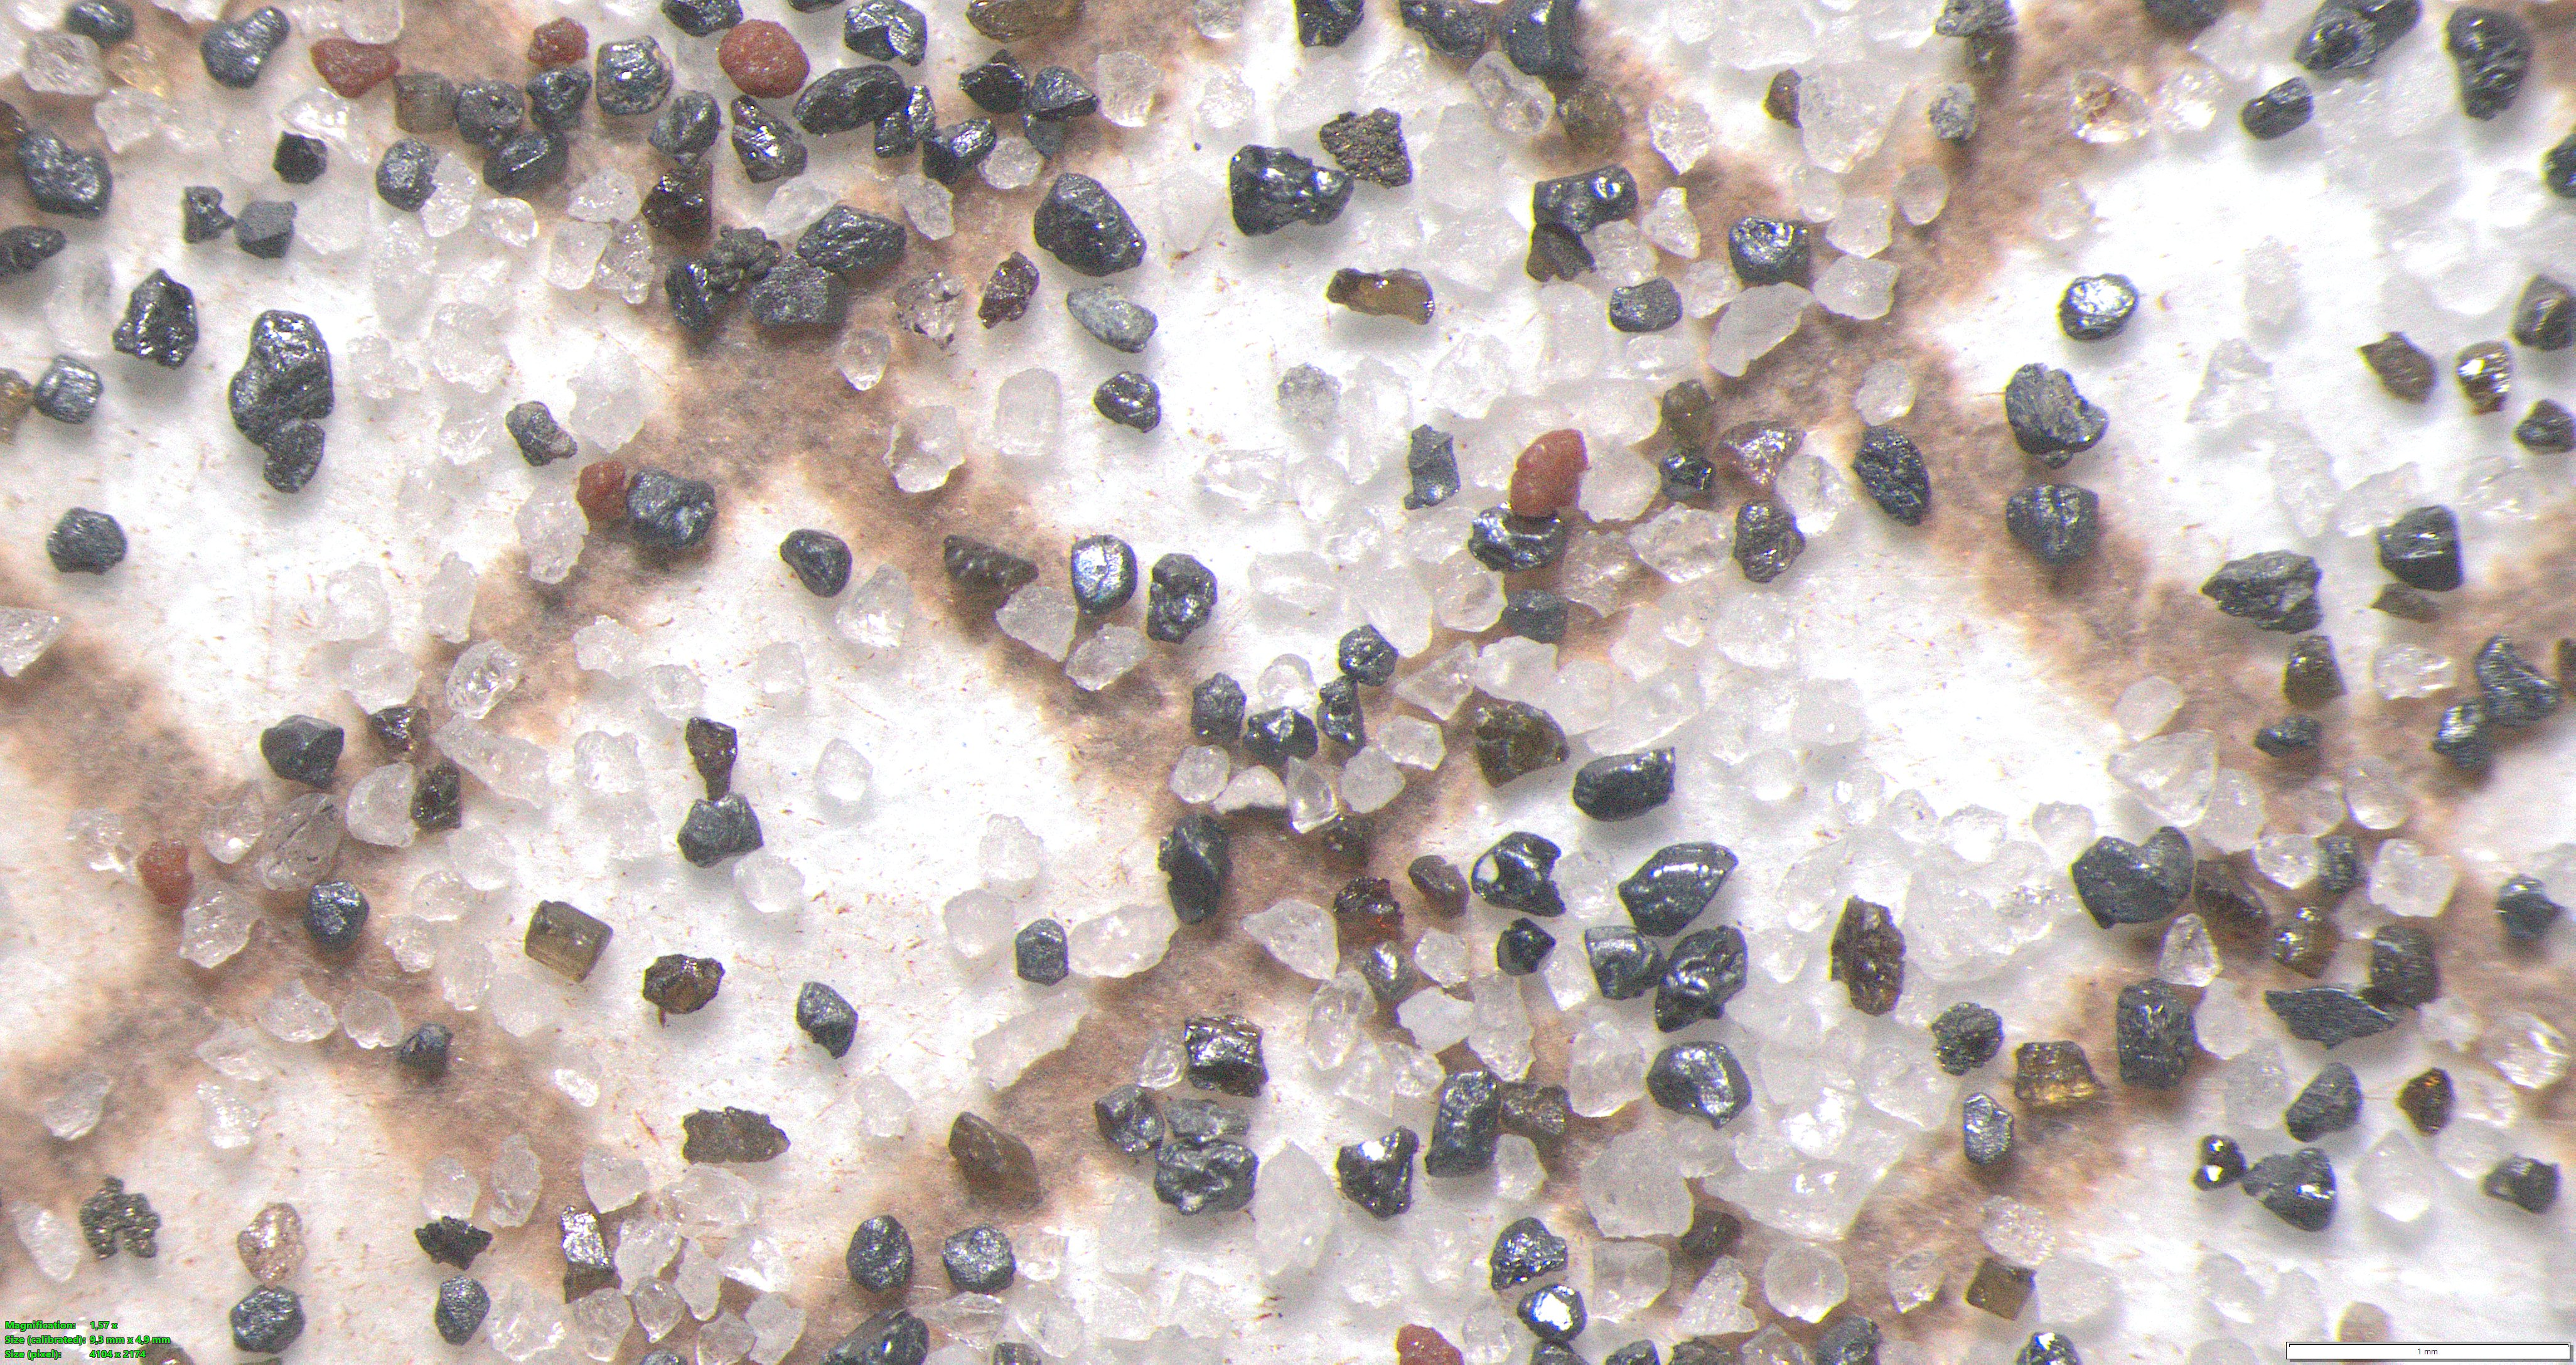
\includegraphics[width=\textwidth]{figure/micSedang.jpg}
        \caption{Kecerahan Citra Mikroskop Optimal}
        \label{fig:2.Mic2}
    \end{subfigure}
    
    \caption{Perbandingan Tingkat Kecerahan Citra Mikroskop}
    \label{fig:2.MicComparison}
\end{figure}

\subsubsection{Ruang Warna RGB} \label{II.Ruang-Warna-RGB}
Citra berwarna, yang sering dikenal dengan istilah truecolor, menggunakan ruang warna RGB untuk menyajikan data visual melalui penggabungan tiga komponen dasar yaitu Merah (Red), Hijau (Green), dan Biru (Blue). Model ini diadopsi secara luas pada perangkat seperti monitor dan kamera video karena reseptor mata manusia dapat merasakan kombinasi ketiga warna ini secara efektif untuk membentuk persepsi visual. Secara teknis, setiap komponen warna dalam sistem ini menggunakan kedalaman 8 bit yang menentukan intensitasnya dalam rentang nilai 0 hingga 255. Dengan variasi intensitas tersebut, ruang warna RGB memungkinkan representasi spektrum yang sangat luas hingga mencapai total 16.581.375 kemungkinan warna yang dapat disajikan \cite{bookCitra}. \par

\subsection{Prapemrosesan Data} \label{II.TeoriPrapemrosesan}
Prapemrosesan data (\textit{data preprocessing}) merupakan tahap awal dalam pengolahan data yang bertujuan untuk meningkatkan kualitas data sebelum data tersebut digunakan ke dalam model. Tahap ini dilaksanakan karena dalam banyak kasus data mentah yang akan digunakan, termasuk pada data yang seringkali mengalami masalah seperti ukuran (dimensi) yang tidak konsisten, orientasi atau posisi objek yang berbeda-beda, skala nilai yang tidak seragam, maupun format atau pencahayaan yang variatif. Dengan melakukan prapemrosesan, data menjadi lebih konsisten, mudah diolah, dan model yang dibangun memiliki peluang konvergensi yang lebih baik serta mampu menghasilkan generalisasi yang lebih baik. \par

\subsubsection{Segmentasi Citra} \label{II.TeoriSegmentasiCitra}
Segmentasi citra adalah proses fundamental dalam pemprosesan citra digital dan visi komputer yang bertujuan mempartisi atau membagi citra menjadi beberapa segmen atau subkelompok piksel, yang sering disebut sebagai \textit{region} atau objek \cite{imageSegmentation} \cite{bookCitra}. Secara teknis, segmentasi melibatkan pemberian label unik pada setiap piksel dalam citra sedemikian rupa sehingga piksel-piksel dengan label yang sama berbagi karakteristik visual tertentu (seperti warna, intensitas, atau tekstur) dan secara kolektif membentuk suatu \textit{region} yang koheren \cite{bookCitra}. 
Segmentasi citra terbagi menjadi semantic segmentation, yaitu pelabelan piksel berdasarkan kategori objek hanya sesama kelas, dan instance segmentation, yang tidak hanya mengelompokkan berdasarkan kategori tetapi juga membedakan setiap objek individual dari kelas yang sama \cite{imageSegmentation}. Hasil segmentasi pada Gambar \ref{fig:2.SegmentasiComparison} diperoleh menggunakan metode \textit{instance segmentation}, yang mampu mengidentifikasi dan memberi label pada setiap objek secara individual.\par

\begin{figure}[H]
	\centering
	% Baris pertama: dua gambar sejajar
	\begin{subfigure}[b]{0.425\textwidth}
		\centering
		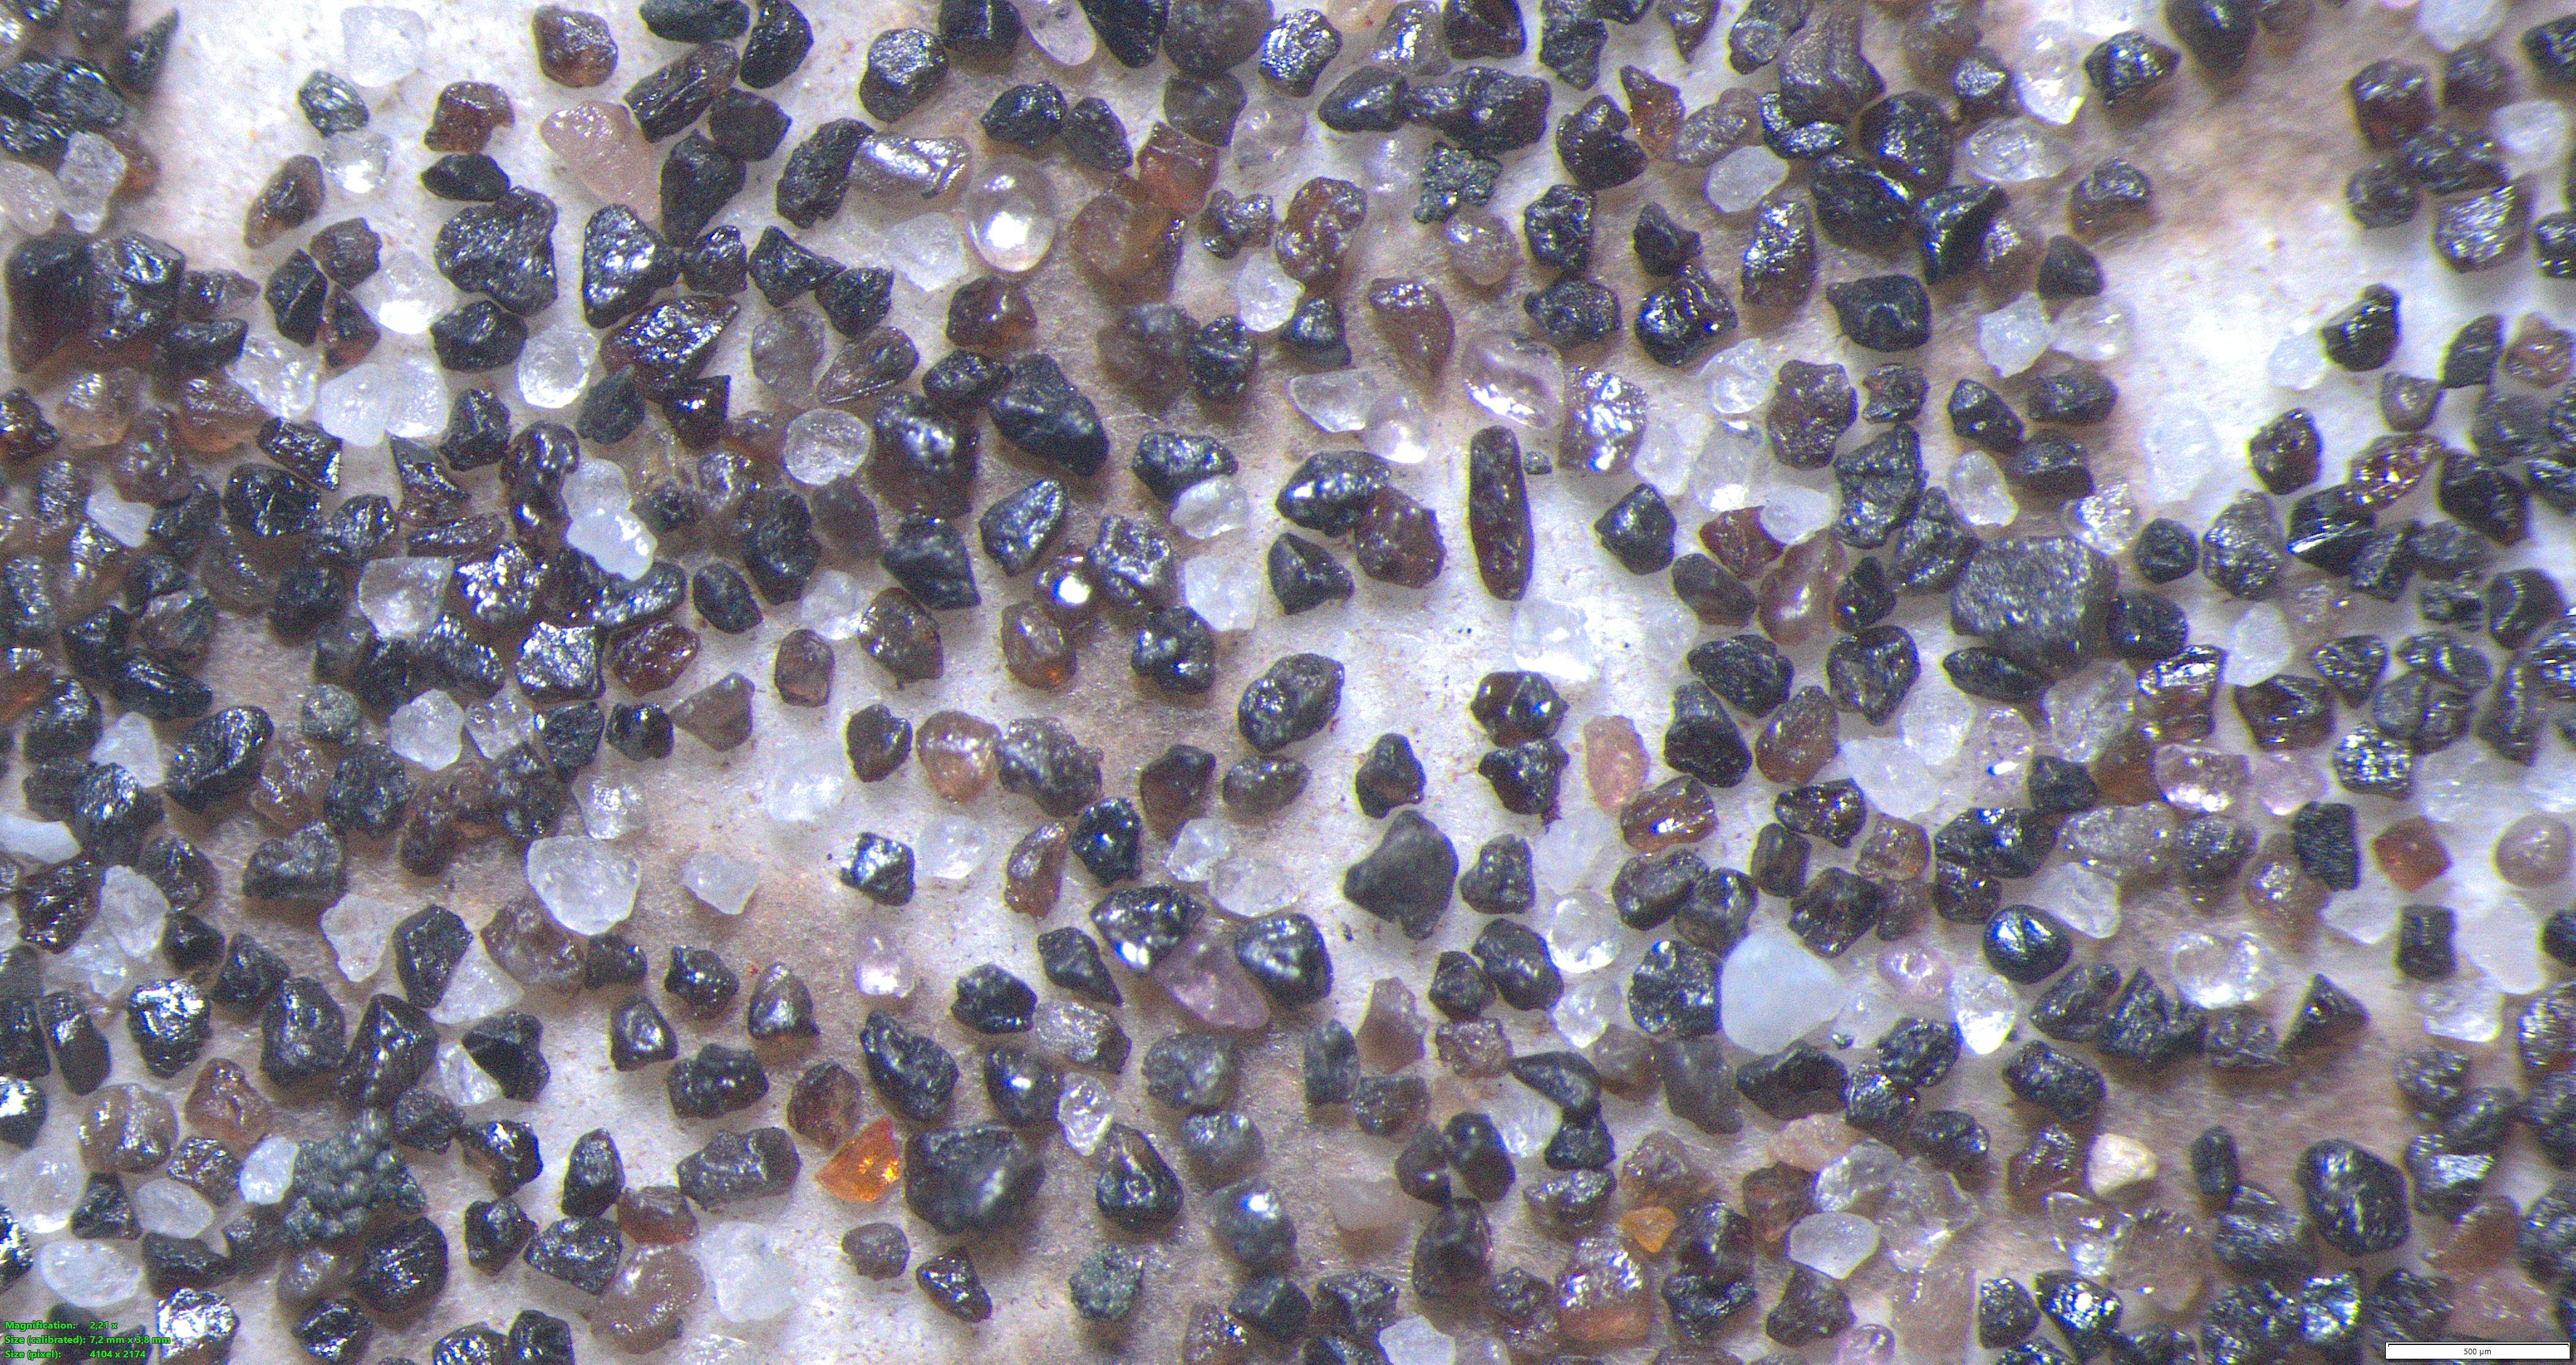
\includegraphics[width=\textwidth]{figure/segmentasiOri.jpg}
		\caption{Citra Original}
		\label{fig:2.Segmentasi1}
	\end{subfigure}
	\hspace{0.5cm}
	\begin{subfigure}[b]{0.425\textwidth}
		\centering
		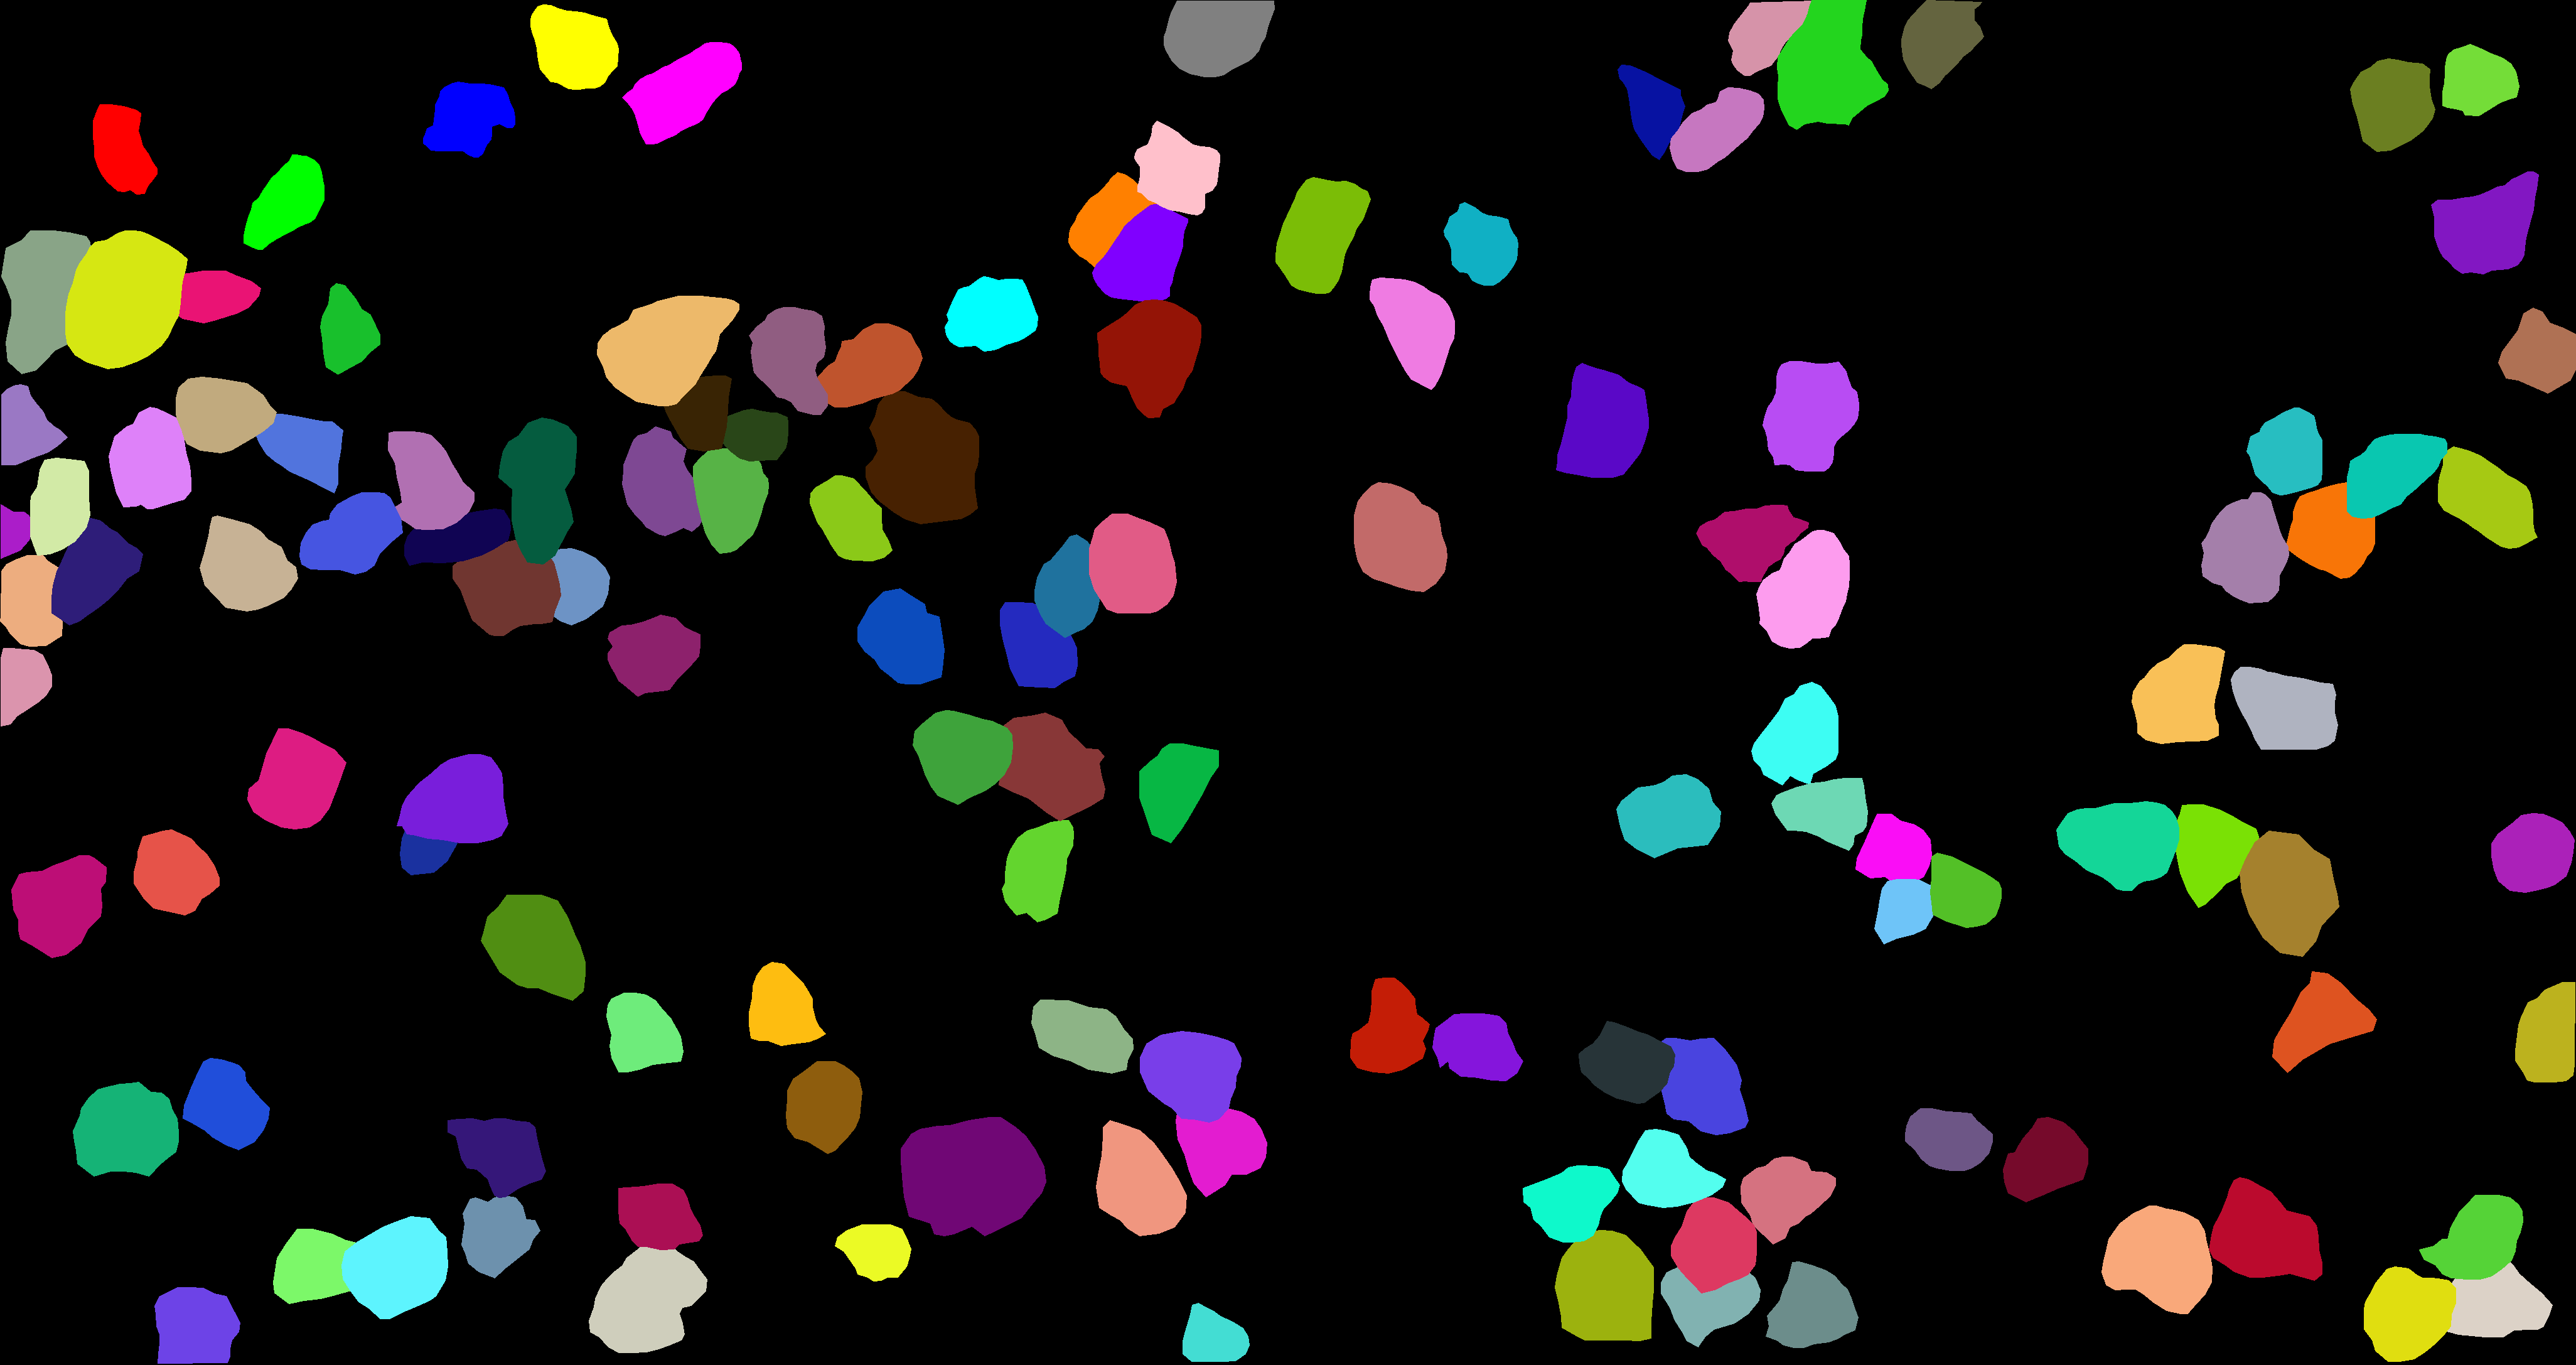
\includegraphics[width=\textwidth]{figure/segmentasiMask.png}
		\caption{Citra Hasil Segmentasi (\textit{Mask})}
		\label{fig:2.Segmentasi2}
	\end{subfigure}

	\caption{Perbandingan Hasil Segmentasi Citra}
	\label{fig:2.SegmentasiComparison}
\end{figure}

\subsubsection*{\textnormal{1. \textit{Amodal Instance Segmentation}}}
 \label{II.TeoriAmodalInstanceSegmentation}
\textit{Amodal instance segmentation} merupakan tugas untuk memprediksi wilayah yang mencakup keseluruhan bagian objek, baik yang terlihat (\textit{visible}) maupun yang terhalang atau tersembunyi (\textit{occluded}) oleh objek lain. Ini berbeda dari \textit{modal instance segmentation} standar, yang tujuannya hanya menandai piksel-piksel objek yang terlihat. Tantangan utama dalam pengembangan metode untuk tugas ini adalah kurangnya ketersediaan data latih publik yang memiliki anotasi \textit{amodal}. Meskipun demikian, sebuah sistem segmentasi \textit{amodal} yang efektif sangat penting karena memungkinkan penalaran oklusi (\textit{occlusion reasoning}) yang canggih, seperti kemampuan untuk menyimpulkan keberadaan, batasan, dan urutan kedalaman relatif dari objek yang terhalang \cite{AmodalInstanceSegmentation}. Perbandingan citra asli dengan hasil segmentasi \textit{modal} dan \textit{amodal} ditunjukkan pada Gambar \ref{fig:2.Amodal}, yang menggambarkan perbedaan area prediksi antara objek yang terlihat dan yang tersembunyi. \par

\begin{figure}[H] % Kalau menggunakan H, posisi gambar akan tepat dibawah teks
    \centering
    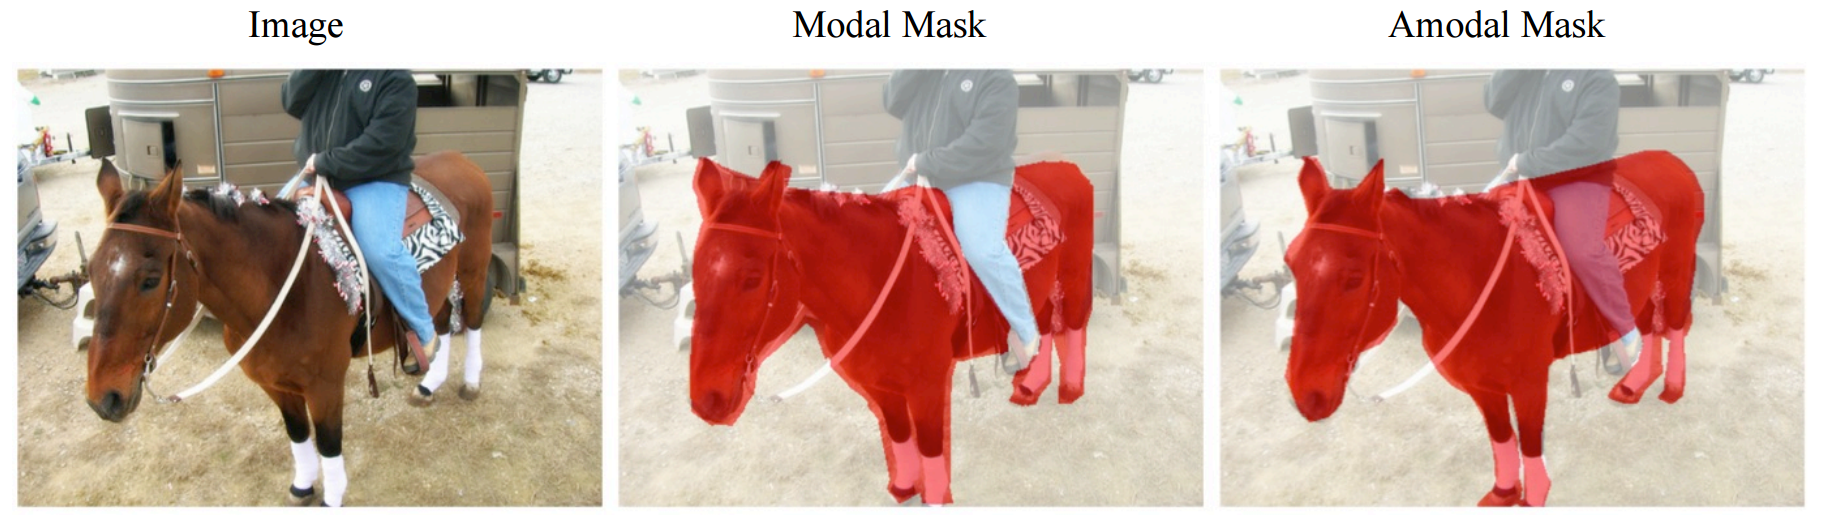
\includegraphics[width=1\textwidth]{figure/amodal.png}
    \caption{Perbandingan Hasil Segmentasi \textit{modal} dan \textit{amodal} \cite{AmodalInstanceSegmentation}}
    \label{fig:2.Amodal}
\end{figure}

\subsubsection{Pembagian Citra (\textit{Image Tiling})} \label{II.TeoriImageTiling}
Pembagian citra (\textit{image tiling}) merupakan teknik strategi pemrosesan yang membagi citra beresolusi tinggi menjadi potongan-potongan sub-citra (\textit{tiles}) yang saling tumpang tindih untuk mengatasi hilangnya detail pada deteksi objek kecil. Pendekatan ini secara efektif meningkatkan ukuran area piksel relatif objek kecil saat dimasukkan ke dalam jaringan saraf tiruan, sehingga mencegah kegagalan deteksi yang sering terjadi akibat proses \textit{down-sampling} pada arsitektur CNN standar. Metode ini diterapkan secara konsisten baik pada tahapan pelatihan (\textit{training}) untuk memperkaya representasi data, maupun pada tahapan inferensi (\textit{inference}) untuk menjaga akurasi deteksi pada perangkat dengan daya komputasi terbatas seperti GPU seluler. Akhirnya, proposal objek yang terdeteksi secara independen pada setiap potongan citra akan digabungkan kembali menggunakan algoritma merging yang memperhitungkan irisan antar-\textit{tile} untuk menghasilkan deteksi final yang akurat pada resolusi asli citra \cite{ImageTiling}.

% \subsubsection{\textit{Resize}} \label{II.TeoriResize}
% \textit{Resize image} merupakan salah satu tahap \textit{preprocessing} yang berperan untuk menyamaratakan semua gambar pada tingkat ukuran yang sama dengan ukuran yang telah ditentukan (misalnya $1920 \times 1080$) \cite{resize}. Penyesuaian  dimensi  gambar pada tahap ini memastikan bahwa semua data yang akan di input dapat diproses secara konsisten oleh model. Tujuan utama dari penyeragaman ukuran ini adalah untuk mengurangi ukuran file suatu citra dan meringankan beban kerja dari proses training data. 

\subsubsection{Augmentasi Data} \label{II.TeoriAugmentasiData}
Augmentasi data merupakan proses modifikasi gambar dalam dataset untuk menciptakan variasi baru sehingga data menjadi lebih beragam tanpa mengubah label aslinya. Teknik ini bertujuan untuk meningkatkan keragaman data pelatihan secara minimal tanpa perlu mengumpulkan data baru secara manual, yang berfungsi efektif untuk mengurangi risiko overfitting. Melalui penambahan variansi data, augmentasi membantu model mengenali pola visual dari berbagai sudut pandang dan skenario pencahayaan yang berbeda.

\subsubsection*{\textnormal{1. \textit{Flip}}} \label{II.TeoriFlip}
\textit{Flip}, atau membalik gambar, merupakan salah satu teknik manipulasi gambar yang dikategorikan sebagai metode augmentasi data dasar (\textit{basic approaches}). Teknik ini termasuk dalam metode augmentasi geometris yang umumnya diterapkan dalam dua bentuk, yaitu \textit{vertical flip} (membalik secara vertikal) dan \textit{horizontal flip} (membalik secara horizontal). Tujuan utama dari penerapan flipping adalah untuk meningkatkan jumlah dan keragaman data pelatihan secara signifikan tanpa mengubah label atau makna sebenarnya dari citra tersebut \cite{flip}. Operasi \textit{flip} dapat di lakukan menggunakan \ref{eq:2.HorizontalFlip} untuk \textit{flip} horizontal dan \ref{eq:2.VerticalFlip} untuk \textit{flip} vertikal \cite{thesisNova}. \par

\vspace{0.5\baselineskip}
\begin{equationcaptioned}[eq:2.HorizontalFlip]{
		I'(x, y) = I(W - 1 - x, y)
	}{
		Operasi \textit{Horizontal Flip}
	}
\end{equationcaptioned}

Keterangan:
\begin{itemize}
\renewcommand\labelitemi{} % menghilangkan simbol bullet
    \item $I'(x, y)$ : nilai piksel setelah dilakukan pembalikan
    \item $I(x, y)$ : nilai piksel asli
    \item $W$ : lebar citra
    \item $W - 1 - x$ : posisi kolom baru setelah dilakukan pembalikan
    \item $y$ : koordinat baris (tidak berubah)
\end{itemize}

\vspace{0.5\baselineskip}
\begin{equationcaptioned}[eq:2.VerticalFlip]{
		I'(x, y) = I(x, H - 1 - y)
	}{
		Operasi \textit{Vertical Flip}
	}
\end{equationcaptioned}

Keterangan:
\begin{itemize}
\renewcommand\labelitemi{} % menghilangkan simbol bullet
    \item $I'(x, y)$ : nilai piksel setelah dilakukan pembalikan
    \item $H$ : tinggi citra
    \item $H - 1 - y$ : posisi baris baru setelah dilakukan pembalikan
    \item $x$ : koordinat kolom (tidak berubah)
\end{itemize}

\subsubsection*{\textnormal{2. \textit{Rotate}}} \label{II.TeoriRotate}
\textit{Rotate} atau rotasi merupakan metode augmentasi data yang memutar citra pada sudut tertentu, seperti 15°, atau secara acak dalam rentang tertentu. Tujuannya adalah agar model menjadi lebih fleksibel dalam mengenali objek dari melakukan pengenalan pola visual di berbagai orientasi tanpa bergantung pada posisi aslinya. \textit{Rotate} membantu model mengenali pola yang sama meskipun tampil dari sudut pandang berbeda. Dengan demikian, teknik ini meningkatkan kemampuan generalisasi model terhadap variasi orientasi objek pada data pelatihan \cite{RotateBatik}. Operasi \textit{Rotate} dapat dilakukan menggunakan \ref{eq:2.operasi}, di mana matriks rotasi ${R}_\theta$ memutar vektor posisi ${x}$ sebesar sudut $\theta$ untuk menghasilkan posisi baru ${x}'$ setelah rotasi.\par

\vspace{0.5\baselineskip}
\begin{equationcaptioned}[eq:2.operasi]{
		{x}' = {R}_\theta \, {x}
	}{
		Operasi \textit{Rotate}
	}
\end{equationcaptioned}

Keterangan:
\begin{itemize}
\renewcommand\labelitemi{} % menghilangkan simbol bullet
	\item ${x}'$ : vektor posisi hasil rotasi setelah dilakukan perputaran sebesar sudut $\theta$
    \item ${R}_\theta$ : operator rotasi (matriks rotasi) yang memutar semua titik terhadap titik asal $(0,0)$ sebesar sudut $\theta$
    \item ${x}$ : vektor posisi awal suatu titik atau piksel sebelum rotasi
\end{itemize}

% \vspace{0.5\baselineskip}
% \begin{equationcaptioned}[eq:2.clockwise]{
% 		{R}_{\text{CW}} =
% 		\begin{bmatrix}
% 		\cos\theta & \sin\theta \\
% 		-\sin\theta & \cos\theta
% 		\end{bmatrix}
% 	}{
% 		Operasi \textit{Rotate Clockwise}
% 	}
% \end{equationcaptioned}

% Keterangan:
% \begin{itemize}
% \renewcommand\labelitemi{} % menghilangkan simbol bullet
% 	\item ${R}_{\text{CW}}$ : matriks rotasi untuk arah searah jarum jam (\textit{clockwise})
%     \item $\theta$ : sudut rotasi (dalam radian), searah jarum jam (\textit{clockwise})
% \end{itemize}

% \vspace{0.5\baselineskip}
% \begin{equationcaptioned}[eq:2.counter-clockwise]{
% 		{R}_{\text{CCW}} =
% 		\begin{bmatrix}
% 		\cos\theta & -\sin\theta \\
% 		\sin\theta & \cos\theta
% 		\end{bmatrix}
% 	}{
% 		Operasi \textit{Rotate Counter Clockwise}
% 	}
% \end{equationcaptioned}

% Keterangan:
% \begin{itemize}
% \renewcommand\labelitemi{} % menghilangkan simbol bullet
% 	\item ${R}_{\text{CCW}}$ : matriks rotasi untuk berlawanan arah jarum jam (\textit{counter-clockwise})
%     \item $\theta$ : sudut rotasi (dalam radian), berlawanan arah jarum jam (\textit{counter-clockwise})
% \end{itemize}


\subsubsection*{\textnormal{3. \textit{Gaussian Noise}}} \label{II.TeoriGaussianNoise}
\textit{Gaussian noise} adalah derau statistik (\textit{statistical noise}) yang memiliki fungsi kepadatan probabilitas (\textit{probability density function}) yang setara dengan distribusi normal. Derau ini bersifat aditif (\textit{additive noise}), di mana piksel dalam gambar yang bising (\textit{noisy image}) merupakan hasil penjumlahan dari nilai piksel asli dengan nilai \textit{Gaussian noise} acak. \textit{Gaussian noise} bersifat independen di setiap piksel dan juga independen terhadap besaran sinyal (\textit{signal magnitude}) \cite{GaussianNoiseManga}. Dalam konteks augmentasi data, Gaussian noise dapat ditambahkan ke fitur kueri (\textit{query feature}) yang diambil sampelnya dari distribusi \textit{Gaussian} untuk meningkatkan variasi kueri tersebut di dalam \textit{feature space} \cite{GaussianNoise}. Operasi \textit{Gaussian Noise} dapat di lakukan menggunakan \ref{eq:2.gaussian_distribution} untuk distribusi \textit{gaussian} pada fitur \par
% dan \ref{eq:2.gaussian_addition} untuk penambahan noise ke fitur yang hanya di lakukan pada tahap \textit{training} untuk memperbesar variasi data di ruang fitur.\par

\vspace{0.5\baselineskip}
\begin{equationcaptioned}[eq:2.gaussian_distribution]{
    n_{ijk} \sim \mathcal{N}(0, \sigma_i^2)
}{
    Distribusi \textit{Gaussian} pada Fitur
}
\end{equationcaptioned}

Keterangan:
\begin{itemize}
\renewcommand\labelitemi{} % menghilangkan simbol bullet
    \item $n_{ijk}$ : nilai \textit{noise} pada channel ke-$i$, baris ke-$j$, dan kolom ke-$k$
    \item $\sigma_i$ : standar deviasi dari \textit{noise} untuk channel ke-$i$
    \item $\mathcal{N}(0, \sigma_i^2)$ : distribusi Gaussian dengan mean $0$ dan variansi $\sigma_i^2$
\end{itemize}

% \vspace{0.5\baselineskip}
% \begin{equationcaptioned}[eq:2.gaussian_addition]{
%     {F}_q \leftarrow {F}_q + {N}
% }{
%     Penambahan \textit{Noise Gaussian} pada Fitur
% }
% \end{equationcaptioned}

% Keterangan:
% \begin{itemize}
% \renewcommand\labelitemi{} % menghilangkan simbol bullet
%     \item ${F}_q$ : fitur dari \textit{query image}
%     \item ${N}$ : tensor \textit{Gaussian noise} berukuran $C \times H \times W$
% \end{itemize}

\subsubsection{\textit{Normalization}} \label{II.TeoriNormalization}
\textit{Normalization} atau proses normalisasi adalah sebuah proses mengubah nilai piksel pada gambar ke dalam rentang tertentu, seperti melakukan konversi nilai piksel dari rentang 0--255 menjadi 0--1. Proses ini digunakan untuk mempersiapkan data agar dapat memenuhi kebutuhan pemrosesan dan mendukung model dalam mendapatkan hasil yang lebih optimal. Pentingnya proses normalisasi adalah agar input memiliki nilai yang seragam. Input data yang tidak seragam akan mempengaruhi proses komputasi dan hasil akhir pada aplikasi \cite{Normalisasi}. Operasi normalisasi piksel dapat dilakukan dengan menggunakan \ref{eq:2.normalization} \cite{thesisNova}. \par

\vspace{0.5\baselineskip}
\begin{equationcaptioned}[eq:2.normalization]{
    X_{normal} = \frac{X - X_{min}}{X_{max} - X_{min}}
}{
    Normalisasi Piksel
}
\end{equationcaptioned}

Keterangan:
\begin{itemize}
\renewcommand\labelitemi{} % menghilangkan simbol bullet
    \item $X_{normal}$ : nilai piksel setelah dilakukan normalisasi
    \item $X_{min}$ : nilai piksel minimum dalam citra (biasanya 0)
    \item $X_{max}$ : nilai piksel maksimum dalam citra (biasanya 255)
    \item $X$ : nilai piksel asli
\end{itemize}

\subsection{\textit{Deep Learning}} \label{II.TeoriDeepLearning}
\textit{Deep Learning} merupakan metode pembelajaran representasi yang menggunakan model komputasi dengan beberapa lapisan pemrosesan untuk mempelajari representasi data pada berbagai tingkat abstraksi. Metode ini memungkinkan mesin untuk diberi data mentah dan secara otomatis menemukan representasi yang diperlukan untuk deteksi atau klasifikasi. Dimulai dari input mentah, setiap modul sederhana namun \textit{non-linear} dalam lapisan tersebut mengubah representasi di satu tingkat menjadi representasi di tingkat yang lebih tinggi dan sedikit lebih abstrak \cite{DeepLearning}. \par

Untuk menemukan struktur rumit dalam kumpulan data besar, \textit{deep Learning} memanfaatkan algoritma backpropagation untuk menunjukkan bagaimana mesin harus mengubah parameter internalnya di setiap lapisan. Aspek kunci dari \textit{deep Learning} adalah bahwa lapisan-lapisan fitur ini tidak dirancang oleh insinyur manusia, melainkan dipelajari dari data menggunakan prosedur pembelajaran umum. Pendekatan ini telah secara dramatis meningkatkan kemampuan \textit{state-of-the-art} dalam berbagai \textit{domain}, termasuk klasifikasi gambar, pengenalan objek visual, deteksi objek, dan pengenalan ucapan \cite{DeepLearning} \cite{DeepResidual}. \par

\subsection{\textit{Transfer Learning}} \label{II.TeoriTransferLearning}
\textit{Transfer learning} merupakan sebuah pendekatan yang memanfaatkan pengetahuan (\textit{knowledge}) dari domain sumber untuk meningkatkan kinerja pada domain target. Pendekatan ini sering menggunakan \textit{pre-trained model}, yaitu model yang telah dilatih pada dataset berskala besar sehingga menyediakan pengetahuan dasar dan umum yang fundamental untuk tugas-tugas \textit{downstream}. Dengan memanfaatkan model yang sudah dilatih ini, sebuah paradigma yang sukses seperti \textit{fine-tuning} memungkinkan peningkatan kinerja pada tugas target tanpa harus memulai keseluruhan proses pelatihan dari awal. Karena banyaknya model yang tersedia, penilaian \textit{pre-trained model} untuk \textit{transfer learning} menjadi penting untuk mengidentifikasi kandidat model yang optimal bagi tugas \textit{downstream} tertentu \cite{TransferLearning}. \par

\subsection{\textit{Mask} R-CNN} \label{II.TeoriMaskRCNN}
\textit{Mask} R-CNN adalah sebuah kerangka kerja (\textit{framework}) yang fleksibel dan umum untuk tugas \textit{instance segmentation} objek, yang secara efisien mendeteksi objek dalam sebuah citra dan menghasilkan masker segmentasi berkualitas tinggi untuk setiap objek secara bersamaan \cite{MaskRcnnIEEE11}. Arsitektur ini merupakan perluasan dari \textit{Faster} R-CNN dengan menambahkan sebuah cabang (\textit{branch}) baru secara paralel untuk memprediksi masker objek di samping cabang yang sudah ada untuk klasifikasi kelas dan regresi \textit{bounding box} \cite{MaskRcnnIEEE11}. Alur kerja dan hubungan antar komponen utama seperti \textit{Region Proposal Network} (RPN), \textit{ROI Align}, serta cabang klasifikasi, regresi, dan prediksi masker dapat dilihat pada Gambar \ref{fig:2.MaskR-CNN}.  \par

\begin{figure}[H] % Kalau menggunakan H, posisi gambar akan tepat dibawah teks
    \centering
    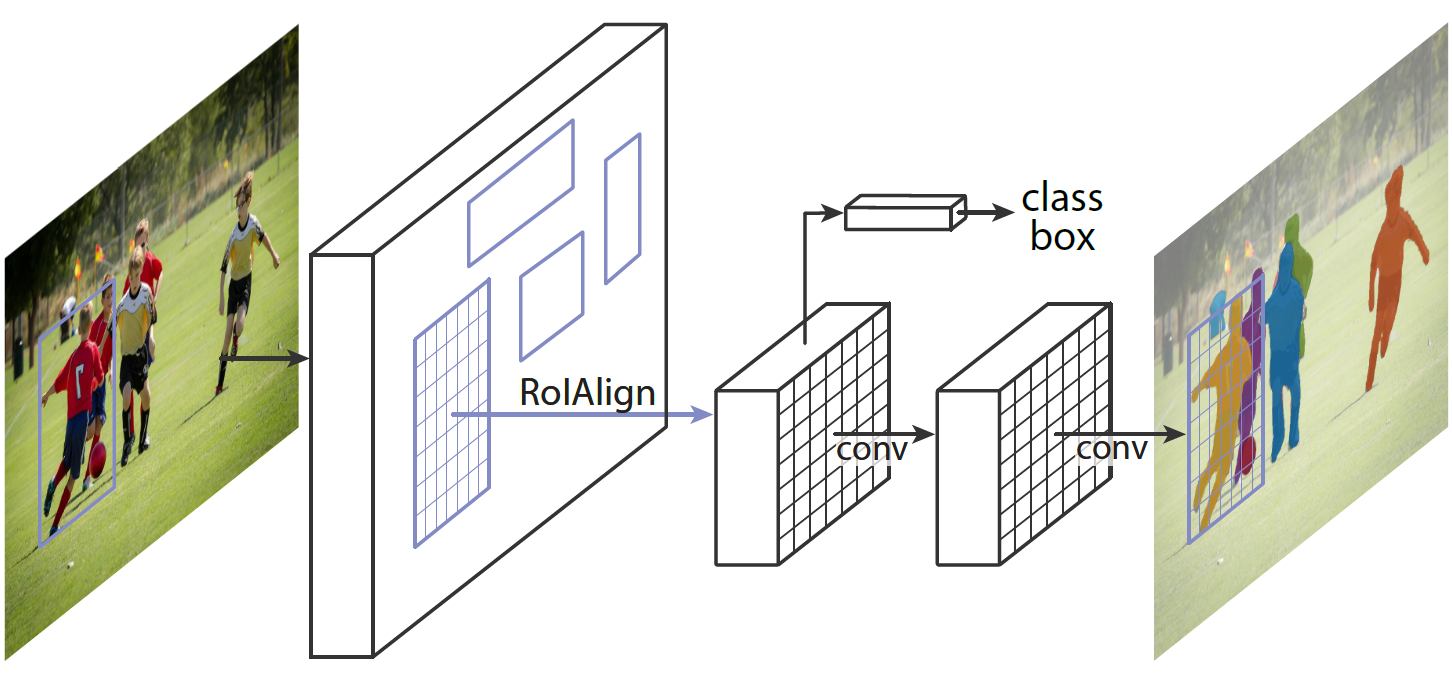
\includegraphics[width=0.8\textwidth]{figure/maskrcnn.png}
    \caption{Alur Kerja dari Arsitektur \textit{Mask} R-CNN \cite{MaskRcnnIEEE11}}
    \label{fig:2.MaskR-CNN}
\end{figure}

Pendekatan \textit{Mask} R-CNN ini mengikuti prosedur dua tahap yang sama seperti \textit{Faster} R-CNN, dimana tahap pertama adalah RPN yang mengusulkan kandidat \textit{bounding box} objek, dan tahap kedua secara paralel melakukan klasifikasi, regresi \textit{bounding box}, serta prediksi masker biner untuk setiap RoI \cite{MaskRcnnIEEE11}. Secara arsitektur, \textit{Mask} R-CNN dimulai dengan jaringan \textit{backbone} konvolusi (seperti ResNet yang dikombinasikan dengan \textit{Feature Pyramid Network} (FPN)) yang berfungsi untuk mengekstraksi fitur dari seluruh citra input. Fitur yang diekstraksi kemudian diteruskan ke RPN untuk menghasilkan sejumlah kandidat RoI \cite{MaskRcnnIEEE11}. Setiap RoI diproses melalui lapisan RoIAlign guna menjaga keselarasan spasial sebelum diteruskan ke tiga cabang paralel untuk klasifikasi objek, regresi \textit{bounding box}, dan prediksi masker biner berukuran $m \times m$ untuk setiap kelas objek \cite{MaskRcnnIEEE11}. Fungsi kerugian total (\textit{loss function}) pada \textit{Mask} R-CNN dapat dilihat pada \ref{eq:2.maskrcnn} \cite{MaskRcnnIEEE11}, yang merupakan gabungan dari tiga komponen kerugian utama. Perhitungan \textit{classification loss} secara spesifik ditunjukkan pada Persamaan~\ref{eq:2.cls_loss}, sedangkan perhitungan \textit{bounding box regression loss} dijelaskan pada Persamaan~\ref{eq:2.box_loss}, dan perhitungan \textit{mask loss} secara spesifik dijelaskan pada \ref{eq:2.maskloss} \cite{rumusMaskrcnn} berikut. \par

\vspace{0.5\baselineskip}
\begin{equationcaptioned}[eq:2.maskrcnn]{
	L = L_{\text{cls}} + L_{\text{box}} + L_{\text{mask}}
}{
	Fungsi Loss \textit{Mask} R-CNN
}
\end{equationcaptioned}

Keterangan:
\begin{itemize}
\renewcommand\labelitemi{} % menghilangkan simbol bullet
	\item \(L_{\text{cls}}\) : \textit{classification loss} untuk memprediksi kelas objek.
	\item \(L_{\text{box}}\) : \textit{bounding box regression loss} untuk memperkirakan posisi kotak pembatas.
	\item \(L_{\text{mask}}\) : \textit{mask loss} berbasis \textit{binary cross-entropy} yang dihitung per piksel pada setiap \textit{Region of Interest (RoI)}.
\end{itemize}

\vspace{0.5\baselineskip}
\begin{equationcaptioned}[eq:2.cls_loss]{
    {L}_{cls}
    = \frac{1}{N_{cls}} \sum_i \big(-p_i^* \log p_i - (1 - p_i^*) \log (1 - p_i)\big)
}{
    Fungsi kerugian klasifikasi (\textit{Classification Loss})
}
\end{equationcaptioned}

Keterangan:
\begin{itemize}
\renewcommand\labelitemi{} % menghilangkan simbol bullet
    \item ${L}_{cls}$ : \textit{Classification loss}, menghitung kesalahan antara hasil klasifikasi ($p_i$) dan label sebenarnya ($p_i^*$).
    \item $N_{cls}$ : Jumlah total \textit{anchor} yang digunakan untuk proses klasifikasi.
    \item $p_i$ : Probabilitas prediksi bahwa \textit{anchor} ke-$i$ mengandung objek (output dari \textit{sigmoid classifier}).
    \item $p_i^*$ : Label kebenaran untuk \textit{anchor} ke-$i$ ($1$ jika mengandung objek, $0$ jika bukan objek).
\end{itemize}

\vspace{0.5\baselineskip}
\begin{equationcaptioned}[eq:2.box_loss]{
    {L}_{box}
    = \frac{\lambda}{N_{box}} \sum_i p_i^* \cdot L_1^{smooth}(t_i - t_i^*)
}{
    Fungsi kerugian regresi kotak pembatas (\textit{Bounding Box Regression Loss})
}
\end{equationcaptioned}

Keterangan:
\begin{itemize}
\renewcommand\labelitemi{} % menghilangkan simbol bullet
    \item ${L}_{box}$ : \textit{Bounding box regression loss}, mengukur perbedaan antara koordinat prediksi ($t_i$) dan koordinat sebenarnya ($t_i^*$).
    \item $N_{box}$ : Jumlah total \textit{anchor} yang digunakan untuk regresi kotak pembatas.
    \item $t_i$ : Vektor koordinat prediksi kotak pembatas hasil regresi.
    \item $t_i^*$ : Vektor koordinat sebenarnya dari kotak pembatas (\textit{ground truth box}).
    \item $\lambda$ : Koefisien penyeimbang antara kerugian klasifikasi dan regresi.
    \item $L_1^{smooth}$ : \textit{Smooth L1 loss}, fungsi yang digunakan untuk menghitung selisih koordinat secara stabil tanpa pengaruh ekstrem.
\end{itemize}

\vspace{0.5\baselineskip}
\begin{equationcaptioned}[eq:2.maskloss]{
	L_{\text{mask}} = -\frac{1}{m^2}\sum_{1 \leq i,j \leq m}
	\Big[ y_{ij} \log \hat{y}^{k}_{ij} + (1 - y_{ij}) \log (1 - \hat{y}^{k}_{ij}) \Big]
}{
	Operasi \textit{Mask Loss (Binary Cross-Entropy)}
}
\end{equationcaptioned}

Keterangan:
\begin{itemize}
\renewcommand\labelitemi{}
	\item $m$² atau $m \times m$ : ukuran resolusi keluaran \textit{mask} untuk setiap kelas objek.
	\item $y_{ij}$ : nilai \textit{ground-truth} piksel ke-$i,j$ (1 untuk area objek, 0 untuk latar belakang).
	\item $\hat{y}^{k}_{ij}$ : probabilitas hasil prediksi piksel ke-$i,j$ untuk kelas objek ke-$k$.
	\item Operasi penjumlahan $\sum_{1 \leq i,j \leq m}$ : menghitung rata-rata \textit{binary cross-entropy loss} dari seluruh piksel pada mask.
\end{itemize}

\subsubsection{\textit{Backbone}} \label{II.TeoriBackbone}
\textit{Backbone} merupakan jaringan konvolusi dasar yang berfungsi mengekstraksi fitur dari seluruh citra sebelum digunakan oleh komponen lain seperti RPN atau \textit{head} deteksi. Salah satu arsitektur yang umum digunakan sebagai \textit{backbone} adalah ResNet-50 (\textit{Residual Network} dengan 50 lapisan), yang memperkenalkan konsep \textit{residual learning} melalui koneksi pintas (\textit{skip connection}) untuk mengatasi masalah degradasi akurasi pada jaringan yang sangat dalam. ResNet-50 terdiri dari lima tahap konvolusi dengan berbagai kedalaman lapisan residual, yang memungkinkan jaringan untuk mempelajari representasi fitur hierarkis dari tingkat rendah hingga tingkat tinggi. Ketika dikombinasikan dengan FPN, ResNet-50 menghasilkan peta fitur multi-skala yang kaya semantik, sehingga meningkatkan kemampuan deteksi dan segmentasi objek pada berbagai ukuran \cite{DeepResidual}. \par

\subsubsection{\textit{Feature Pyramid Network} (FPN)} \label{II.TeoriFPN}
\textit{Feature Pyramid Network} (FPN) merupakan arsitektur yang dirancang untuk memanfaatkan hierarki fitur multi-skala pada jaringan konvolusi (\textit{backbone}) guna membentuk piramida fitur dengan makna semantik yang konsisten di setiap tingkat skala, namun dengan biaya komputasi yang rendah \cite{fpn}. FPN menggabungkan fitur beresolusi rendah yang kaya semantik dari lapisan dalam dengan fitur beresolusi tinggi yang detail secara spasial dari lapisan dangkal melalui jalur \textit{top-down} dengan \textit{upsampling} dan koneksi lateral menggunakan konvolusi $1 \times 1$ serta penjumlahan \textit{element-wise} \cite{fpn}. Struktur umum dari arsitektur FPN dapat dilihat pada Gambar \ref{fig:2.FPN} yang memperlihatkan alur pembentukan piramida fitur melalui proses \textit{top-down} dan koneksi lateral \cite{fpn}. Fungsi matematis dari arsitektur FPN yang digunakan untuk menentukan level piramida fitur setiap RoI ditunjukkan pada Persamaan \ref{eq:2.fpn}, yang merepresentasikan hubungan antara ukuran objek dengan level \textit{feature map} yang sesuai dalam struktur piramida multi-skala.
\par

\begin{figure}[H] % Kalau menggunakan H, posisi gambar akan tepat dibawah teks
    \centering
    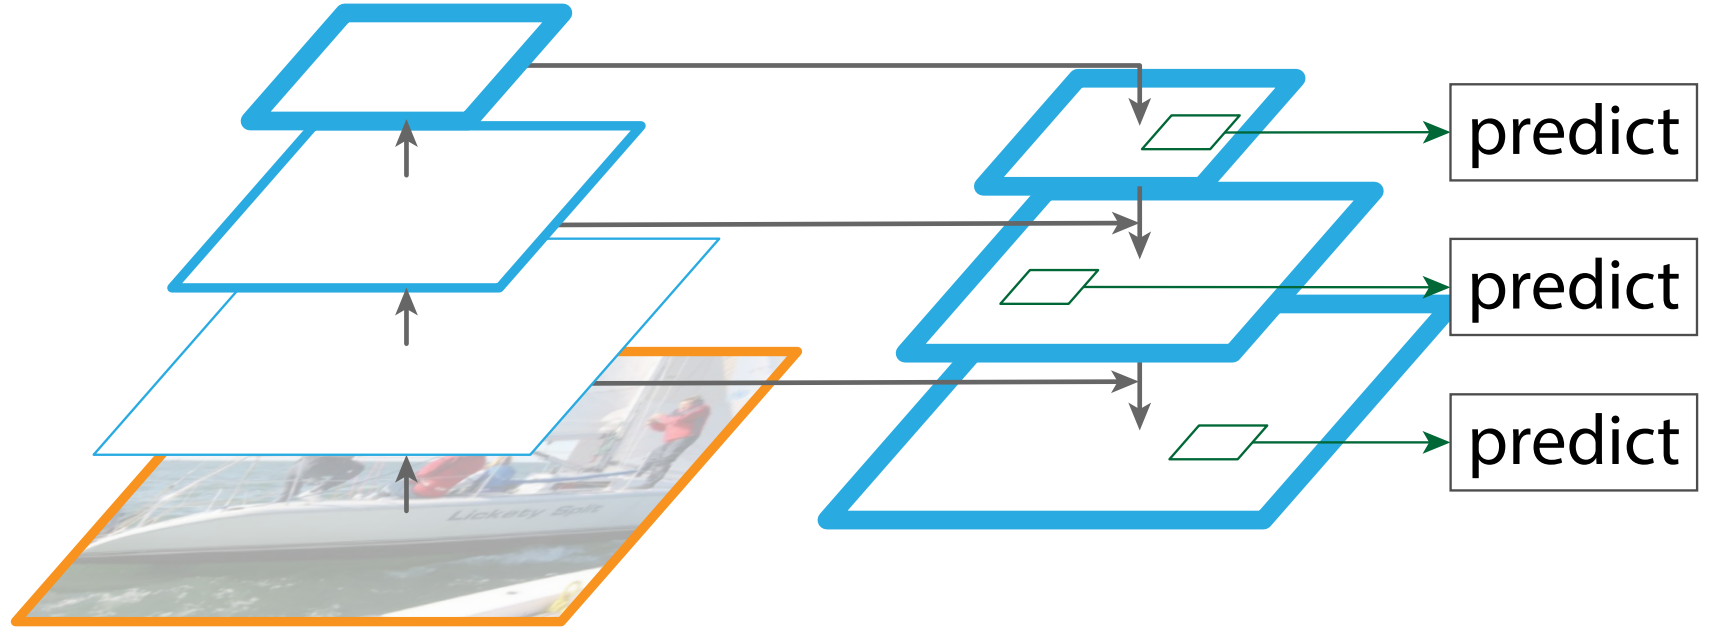
\includegraphics[width=0.8\textwidth]{figure/fpn.png}
    \caption{Arsitektur dari \textit{Feature Pyramid Network} (FPN) \cite{fpn}}
    \label{fig:2.FPN}
\end{figure}

\vspace{0.5\baselineskip}
\begin{equationcaptioned}[eq:2.fpn]{
	k = \left\lfloor k_0 + \log_2\left(\frac{\sqrt{wh}}{224}\right) \right\rfloor
}{
	Operasi Penentuan Level Piramida FPN
}
\end{equationcaptioned}

Keterangan:
\begin{itemize}
\renewcommand\labelitemi{} % menghilangkan simbol bullet
	\item $k$ : level \textit{feature map} piramida ($P_k$) tempat RoI ditempatkan.
	\item $k_0$ : level dasar piramida (biasanya $k_0 = 4$).
	\item $w, h$ : lebar dan tinggi RoI pada citra masukan.
	\item $224$ : ukuran kanonis (\textit{canonical scale}) dari \textit{ImageNet pre-training}, digunakan sebagai skala referensi.
\end{itemize}

% \subsubsection*{\textnormal{1. \textit{Multipath Feature Pyramid Network} (MFPN)}}
%  \label{II.TeoriMFPN}
% \textit{Multipath Feature Pyramid Network} (MFPN) adalah arsitektur jaringan yang diusulkan untuk mengatasi masalah kesalahan identifikasi akibat hilangnya detail fitur lapisan dalam (\textit{deep features}) selama proses ekstraksi fitur. Jaringan ini bekerja dengan menambahkan satu jalur fusi fitur (\textit{feature fusion}) baru dengan arah dari bawah ke atas (\textit{bottom-up}). Jalur baru ini beroperasi secara paralel dengan jalur fusi \textit{top-down} dari FPN orisinal, di mana fitur dari lapisan dangkal (\textit{shallow features}) akan di-downsampling dan ditambahkan ke fitur pada lapisan yang lebih dalam. Fusi dua arah yang paralel ini bertujuan untuk memperkaya informasi detail pada fitur lapisan dalam, sehingga memperkuat kemampuan jaringan dalam mengekstraksi fitur dan meningkatkan akurasi deteksi secara keseluruhan \cite{ImprovedMaskRCNNOrePanggangan}. Struktur umum dari arsitektur MFPN ditunjukkan pada Gambar \ref{fig:2.MFPN}, yang menggabungkan jalur \textit{top-down} dan \textit{bottom-up} secara paralel untuk memperkaya representasi fitur multi-skala melalui proses fusi dua arah yang meningkatkan ketepatan ekstraksi fitur pada lapisan dalam \cite{ImprovedMaskRCNNOrePanggangan}.

% \begin{figure}[H] % Kalau menggunakan H, posisi gambar akan tepat dibawah teks
%     \centering
%     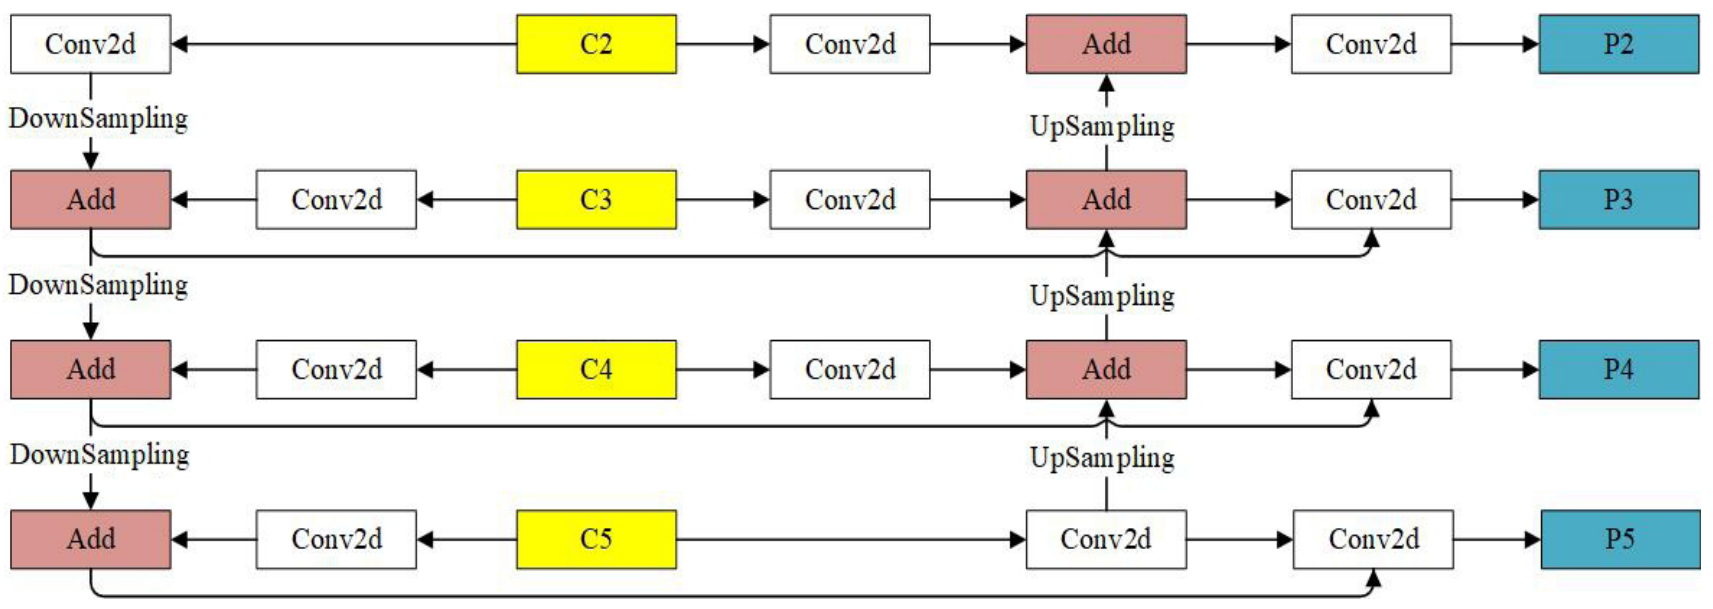
\includegraphics[width=1\textwidth]{figure/MFPN.png}
%     \caption{Struktur Arsitektur \textit{Multipath Feature Pyramid Network} (MFPN) \cite{ImprovedMaskRCNNOrePanggangan}}
%     \label{fig:2.MFPN}
% \end{figure}

\subsubsection{\textit{Region Proposal Network} (RPN)} \label{II.TeoriRPN}
\textit{Region Proposal Network} (RPN) adalah sebuah Jaringan Konvolusi Penuh (\textit{Fully Convolutional Network}) yang diperkenalkan untuk mengatasi hambatan komputasi dalam menghasilkan proposal wilayah pada sistem deteksi objek. RPN bekerja dengan cara berbagi lapisan konvolusi full-image dengan jaringan deteksi utama, sehingga memungkinkan proses penghasilan proposal wilayah menjadi hampir tanpa biaya (\textit{nearly cost-free}). Jaringan ini, seperti yang diilustrasikan pada Gambar \ref{fig:2.RPN}, secara bersamaan memprediksi batas-batas objek (\textit{object bounds}) dan skor keobjekan (\textit{objectness scores}) pada setiap posisi di peta fitur konvolusi. RPN dilatih secara \textit{end-to-end} untuk menghasilkan proposal wilayah berkualitas tinggi yang kemudian digunakan oleh jaringan deteksi untuk melakukan deteksi objek \cite{RPN}. Fungsi kerugian (\textit{loss function}) RPN yang digunakan untuk optimasi jaringan ditunjukkan pada Persamaan \ref{eq:RPNLoss}, yang menggabungkan komponen klasifikasi dan regresi untuk setiap \textit{anchor} yang diproses \cite{RPN}. \par

\begin{figure}[H] % Kalau menggunakan H, posisi gambar akan tepat dibawah teks
    \centering
    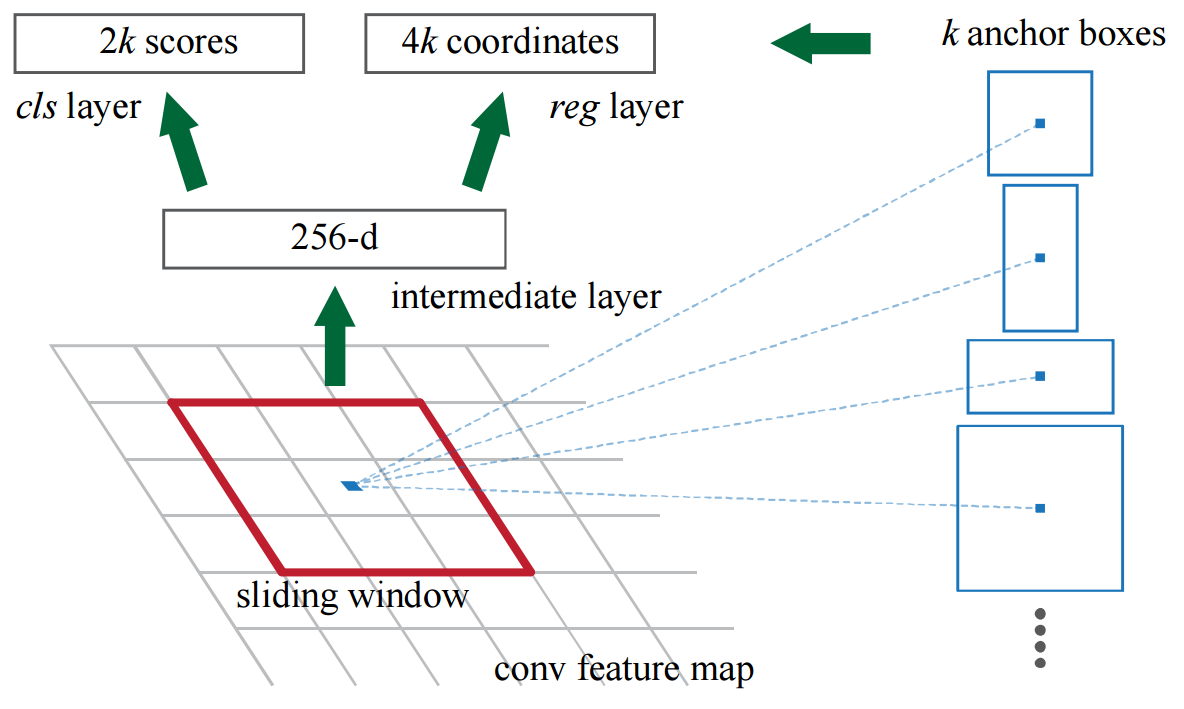
\includegraphics[width=0.8\textwidth]{figure/RPN.png}
    \caption{Jaringan dari \textit{Region Proposal Network} (RPN) \cite{RPN}}
    \label{fig:2.RPN}
\end{figure}

\vspace{0.5\baselineskip}
\begin{equationcaptioned}[eq:RPNLoss]{
    L(\{p_i\}, \{t_i\}) =
    \frac{1}{N_{\text{cls}}} \sum_i L_{\text{cls}}(p_i, p_i^*)
    + \lambda \frac{1}{N_{\text{reg}}} \sum_i p_i^* L_{\text{reg}}(t_i, t_i^*)
}{
    Fungsi Kerugian \textit{loss function} RPN
}
\end{equationcaptioned}

Keterangan:
\begin{itemize}
\renewcommand\labelitemi{} % menghilangkan simbol bullet
    \item $L_{\text{cls}}$ : \textit{Binary Cross-Entropy Loss} yang digunakan untuk membedakan antara \textit{anchor} yang mengandung objek dan yang tidak.
    \item $L_{\text{reg}}$ : \textit{Smooth L1 Loss} yang mengukur perbedaan antara koordinat kotak prediksi dan \textit{ground truth}.
    \item $p_i$ : probabilitas bahwa \textit{anchor} ke-$i$ berisi objek.
    \item $p_i^*$ : label kebenaran untuk \textit{anchor} ke-$i$ (1 jika positif, 0 jika negatif).
    \item $t_i$ : vektor parameter regresi $(t_x, t_y, t_w, t_h)$ hasil prediksi RPN.
    \item $t_i^*$ : vektor target regresi yang dihitung dari selisih antara \textit{anchor} dan \textit{ground truth box}.
    \item $N_{\text{cls}}$ : jumlah total \textit{anchor} dalam satu \textit{mini-batch}.
    \item $N_{\text{reg}}$ : jumlah \textit{anchor} positif yang digunakan untuk regresi.
    \item $\lambda$ : koefisien penyeimbang antara komponen klasifikasi dan regresi (biasanya bernilai 10).
    \item $\sum_i$ : operator penjumlahan yang dilakukan terhadap seluruh \textit{anchor} ke-$i$ pada citra, baik yang berlabel positif maupun negatif.
\end{itemize}
\vspace{0.5\baselineskip}

\subsubsection{\textit{RoIAlign}} \label{II.TeoriRoIAlign}
RoIAlign adalah sebuah lapisan bebas kuantisasi yang dirancang untuk menyelaraskan fitur yang diekstraksi secara tepat dengan input. Prinsip kerjanya adalah menghindari kuantisasi kasar pada koordinat batas-batas RoI ataupun \textit{bin}, misalnya dengan menggunakan $x/16$. Lapisan ini menggunakan \textit{interpolasi bilinear} untuk menghitung nilai-nilai pasti dari fitur input pada empat lokasi sampel yang teratur di dalam setiap \textit{bin} RoI. Nilai-nilai yang dihasilkan kemudian diagregasi (biasanya menggunakan \textit{average} atau \textit{max pooling}) untuk memastikan bahwa fitur yang diekstraksi mempertahankan lokasi spasial yang tepat dan akurat \cite{MaskRcnnIEEE11}. Setiap nilai fitur pada titik $(x, y)$ di dalam \textit{bin} RoI diperoleh dengan menggabungkan empat piksel terdekat secara berbobot menurut jaraknya, yang secara matematis ditunjukkan pada Persamaan~\ref{eq:2.RoIAlign}.


\vspace{0.5\baselineskip}
\begin{equationcaptioned}[eq:2.RoIAlign]{
    y(p) = \sum_{i=0}^{1} \sum_{j=0}^{1} (1 - |x - x_i|)\,(1 - |y - y_j|)\,x(p_{ij})
}{
    Fungsi Interpolasi Bilinear pada \textit{RoIAlign}
}
\end{equationcaptioned}

Keterangan:
\begin{itemize}
\renewcommand\labelitemi{} % menghilangkan simbol bullet
    \item $y(p)$ : nilai fitur hasil \textit{sampling} di titik $(x, y)$ di dalam setiap \textit{bin} RoI.
    \item $x(p_{ij})$ : nilai fitur pada empat piksel terdekat pada \textit{feature map}.
    \item $(x_i, y_j)$ : koordinat piksel integer terdekat terhadap titik $(x, y)$.
    \item $(1 - |x - x_i|)(1 - |y - y_j|)$ : bobot \textit{interpolasi bilinear} yang menentukan kontribusi setiap piksel tetangga.
    \item $\sum_{i=0}^{1} \sum_{j=0}^{1}$ : operasi penjumlahan terhadap empat piksel terdekat untuk mendapatkan nilai fitur interpolasi.
\end{itemize}
\vspace{0.5\baselineskip}

\subsection{\textit{Optimizer}} \label{II.TeoriOptimizer}
\textit{Optimizer} merupakan salah satu komponen matematis utama dalam deep learning yang bertujuan untuk meminimalkan perbedaan antara keluaran yang diharapkan (\textit{expected output}) dan keluaran yang diinginkan (\textit{desired one}), yang diukur melalui \textit{loss function} (fungsi kerugian) \cite{optimizer}. \textit{Optimizer} mencapai tujuan ini secara iteratif dengan mengadaptasi dan memperbarui \textit{weights} (bobot) jaringan berdasarkan nilai kerugian (\textit{loss}) yang dihitung, sebuah proses yang memperkuat algoritma \textit{back-propagation}. Pemilihan \textit{optimizer} yang tepat merupakan keputusan penting karena sangat menentukan kecepatan pelatihan model \textit{deep learning} dan performa akhir yang akan diprediksi oleh model tersebut \cite{optimizer}. \par

% \subsection{\textit{Amodal Segmentation Network} (ASN)} \label{II.TeoriASN}
% \textit{Amodal Segmentation Network} (ASN) merupakan perluasan arsitektur \textit{multi-task} untuk memprediksi bentuk lengkap instan dengan menggabungkan fitur kotak (\textit{box}) dan fitur oklusi (\textit{occlusion}). Jaringan ini memperkenalkan cabang klasifikasi oklusi (\textit{occlusion classification branch}) untuk secara khusus menentukan apakah oklusi ada di dalam \textit{Region of Interest} (RoI). ASN kemudian menggunakan modul \textit{Multi-Level Coding} (MLC) untuk memperkuat informasi global tersebut, menggabungkannya dengan fitur \textit{mask} lokal untuk memandu prediksi segmentasi agar dapat merekonstruksi bagian yang terhalang \cite{AmodalASN}. Struktur umum dari arsitektur \textit{Amodal Segmentation Network} (ASN) dapat dilihat pada Gambar \ref{fig:2.ASN}, yang menunjukkan proses \textit{multi-task} dari ekstraksi fitur hingga segmentasi \textit{amodal} dan \textit{inmodal} \cite{AmodalASN}. Fungsi kerugian total (\textit{loss function}) pada ASN dapat dilihat pada \ref{eq:2.asnloss}, yang merupakan gabungan dari empat komponen kerugian utama. Perhitungan \textit{occlusion loss} secara spesifik ditunjukkan pada Persamaan~\ref{eq:occlusion_loss}, sedangkan perhitungan \textit{mask loss} dijelaskan pada \ref{eq:2.asnmask} berikut. \par

% \begin{figure}[H] % Kalau menggunakan H, posisi gambar akan tepat dibawah teks
%     \centering
%     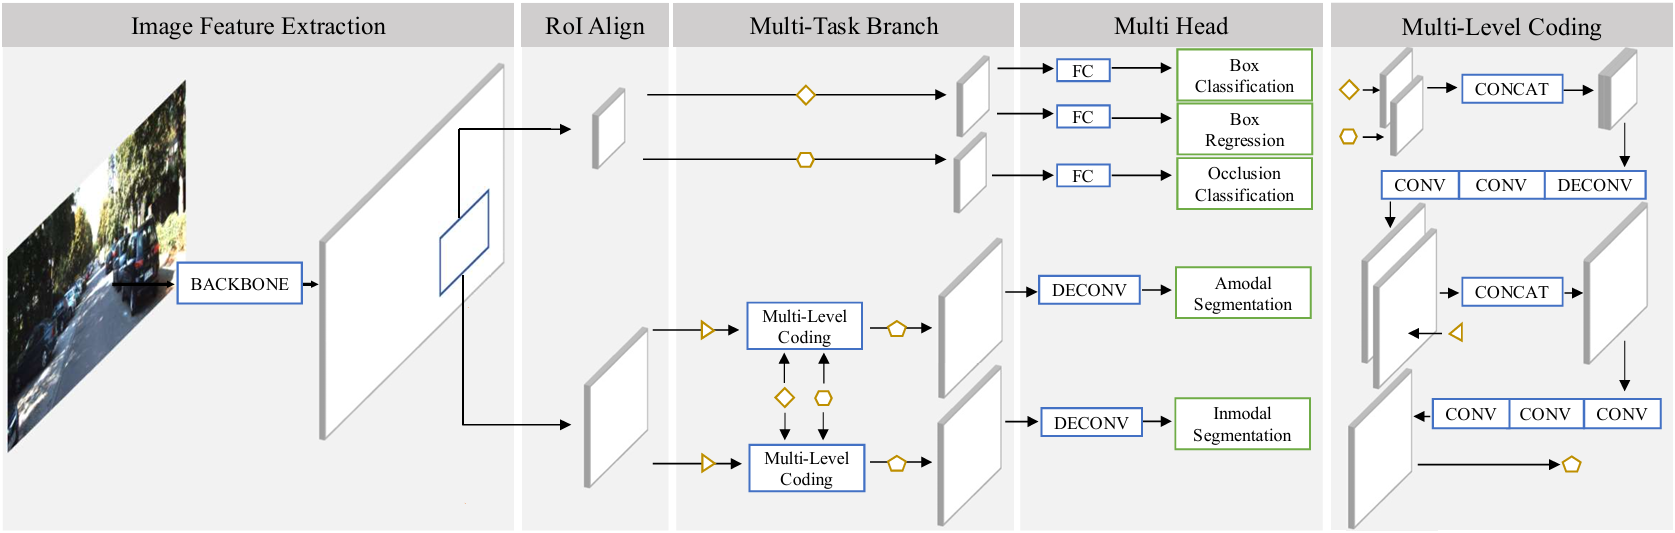
\includegraphics[width=1\textwidth]{figure/asn.png}
%     \caption{Arsitektur ASN hasil modifikasi dari \textit{Mask} R-CNN \cite{AmodalASN}}
%     \label{fig:2.ASN}
% \end{figure}

% \vspace{0.1\baselineskip}
% \begin{equationcaptioned}[eq:2.asnloss]{
% 	L = L_{\text{cls}} + L_{\text{box}} + L_{\text{occlusion}} + L_{\text{mask}}
% }{
% 	Fungsi \textit{Loss} Utama pada ASN
% }
% \end{equationcaptioned}

% Keterangan:
% \begin{itemize}
% \renewcommand\labelitemi{} % menghilangkan bullet
% 	\item \(L_{\text{cls}}\) : \textit{classification loss} untuk memprediksi kelas objek.
% 	\item \(L_{\text{box}}\) : \textit{bounding box regression loss} untuk memperkirakan posisi kotak pembatas.
% 	\item \(L_{\text{occlusion}}\) : \textit{occlusion classification loss} untuk mengenali area tertutup pada citra.
% 	\item $ L_{\text{mask}} $ : penjumlahan dari \textit{binary cross-entropy mask amodal} dan \textit{inmodal}.
% \end{itemize}

% \vspace{0.5\baselineskip}
% \begin{equationcaptioned}[eq:occlusion_loss]{
%     {L}_{occlusion}
%     = -\big[y_{occ} \log(\hat{y}_{occ}) + (1 - y_{occ}) \log(1 - \hat{y}_{occ})\big]
% }{
%     Fungsi kerugian oklusi (\textit{Occlusion Loss})
% }
% \end{equationcaptioned}

% Keterangan:
% \begin{itemize}
% \renewcommand\labelitemi{} % menghilangkan simbol bullet
%     \item ${L}_{occlusion}$ : \textit{Occlusion loss}, mengukur kesalahan klasifikasi dalam menentukan apakah suatu objek tertutupi sebagian (\textit{occluded}) atau terlihat penuh (\textit{visible}).
%     \item $y_{occ}$ : Label kebenaran untuk status oklusi, bernilai $1$ jika objek tertutupi sebagian dan $0$ jika terlihat penuh.
%     \item $\hat{y}_{occ}$ : Nilai probabilitas prediksi model terhadap status oklusi.
%     \item $\log$ : Fungsi logaritma natural yang digunakan untuk menghitung \textit{binary cross-entropy loss}.
% \end{itemize}


% \vspace{0.5\baselineskip}
% \begin{equationcaptioned}[eq:2.asnmask]{
% 	L_{\text{mask}} = L_{\text{mask}}^{a} + L_{\text{mask}}^{i}
% }{
% 	Fungsi \textit{Loss Mask} pada \textit{Amodal} dan \textit{Inmodal Segmentation}
% }
% \end{equationcaptioned}

% Keterangan:
% \begin{itemize}
% \renewcommand\labelitemi{}
% 	\item \(L_{\text{mask}}^{a}\) : \textit{mask loss} untuk segmentasi \textit{amodal} (seluruh bentuk objek).
% 	\item \(L_{\text{mask}}^{i}\) : \textit{mask loss} untuk segmentasi \textit{inmodal} (bagian yang terlihat).
% \end{itemize}

\subsection{\textit{K-Fold Cross Validation}} \label{II.TeoriKFold}
\textit{K-Fold Cross Validation} merupakan sebuah teknik intensif komputasi yang menggunakan semua contoh data yang tersedia, baik sebagai data latih \textit{(train)} maupun data uji \textit{(test)}. Prosedur ini meniru penggunaan \textit{training} dan \textit{test set} dengan melatih algoritma secara berulang sebanyak $K$ kali, di mana setiap kalinya $1/K$ bagian dari data latih disisihkan untuk pengujian \cite{kfold}. Secara praktis, data akan dibagi menjadi $K$ bagian yang terpisah, lalu secara bergantian, satu bagian dipakai untuk tes sementara bagian lainnya dipakai untuk melatih model. Ilustrasi dari \textit{k-fold cross validation} ditampilkan pada Tabel \ref{table:2.KFold}. Hasil akhirnya adalah nilai rata-rata dari semua error yang didapat dari $K$ kali proses pengujian tersebut \cite{kfold}. \par

\begin{table}[H]
\centering
\caption{Ilustrasi \textit{K-Fold Cross Validation}}
\label{table:2.KFold}
\begin{tabular}{|c|c|c|c|c|c|}
\hline
\multirow{2}{*}{\textbf{Iterasi}} & \multicolumn{5}{c|}{\textbf{\textit{K-Fold Cross Validation}}} \\
\cline{2-6}
& \textbf{Fold 1} & \textbf{Fold 2} & \textbf{Fold 3} & \textbf{Fold 4} & \textbf{Fold 5} \\
\hline
1 & \cellcolor{blue!20}\textbf{Test} & Train & Train & Train & Train \\
\hline
2 & Train & \cellcolor{blue!20}\textbf{Test} & Train & Train & Train \\
\hline
3 & Train & Train & \cellcolor{blue!20}\textbf{Test} & Train & Train \\
\hline
4 & Train & Train & Train & \cellcolor{blue!20}\textbf{Test} & Train \\
\hline
5 & Train & Train & Train & Train & \cellcolor{blue!20}\textbf{Test} \\
\hline
\end{tabular}
\end{table}

\subsection{\textit{Average Precision} (AP)} \label{II.TeoriAP}
\textit{Average Precision} (AP) merupakan metrik \textit{de-facto} yang digunakan untuk mengevaluasi kinerja deteksi objek dan segmentasi objek \cite{APmAP}. Secara fundamental, metrik AP dihitung dengan mengukur luas area di bawah kurva \textit{precision-recall detector}, yang secara matematis dapat diekspresikan sebagaimana ditunjukkan pada \ref{eq:2.AP} \cite{ap}. Perhitungan ini mengharuskan setiap prediksi objek memiliki nilai kepercayaan \textit{(confidence value)}, karena evaluasi didasarkan pada pengurutan seluruh prediksi berdasarkan skor kepercayaan tersebut. Sifat metrik ini adalah \textit{rank-sensitive} atau sensitif terhadap peringkat, yang berarti metrik ini memberikan penalti yang lebih besar pada \textit{false positive} (FP) dengan kepercayaan tinggi \textit{(high confidence)} dibandingkan FP dengan kepercayaan rendah \cite{APmAP}. Dengan demikian, nilai AP merupakan rata-rata dari integral kurva \textit{precision-recall} pada berbagai nilai \textit{threshold} IoU. \par

\vspace{0.5\baselineskip}
\begin{equationcaptioned}[eq:2.AP]{
	AP = \frac{1}{|\text{threshold}|} \sum_{\tau \in \text{threshold}} \int_0^1 p(r, \tau)\, dr
}{
	\textit{Average Precision} (AP)
}
\end{equationcaptioned}

Keterangan: 
\begin{itemize}
\renewcommand\labelitemi{} % menghilangkan simbol bullet
	\item $|\text{threshold}|$ : jumlah total nilai \textit{threshold} yang digunakan dalam evaluasi.
	\item $\sum_{\tau \in \text{threshold}}$ : operator penjumlahan yang mengakumulasi nilai AP dari setiap nilai \textit{threshold} IoU yang digunakan.
	\item $\tau$ : nilai \textit{threshold} IoU yang digunakan untuk menentukan apakah prediksi dianggap benar (\textit{true positive}).
	\item $p(r, \tau)$ : nilai \textit{precision} sebagai fungsi dari \textit{recall} ($r$) pada \textit{threshold} $\tau$.
	\item $\int_0^1 p(r, \tau)\, dr$ : integral kurva \textit{precision-recall}, menghitung luas area di bawah kurva untuk \textit{threshold} tertentu.
	\item $dr$ : elemen diferensial yang merepresentasikan perubahan infinitesimal pada nilai \textit{recall}.
\end{itemize}

\subsection{\textit{Intersection over Union} (IoU)} \label{II.TeoriIoU}
\textit{Intersection over Union} (IoU), yang juga dikenal sebagai \textit{Jaccard Index}, merupakan metrik evaluasi yang paling umum digunakan untuk mengukur tingkat kesamaan spasial antara dua objek. IoU melakukan \textit{encoding} terhadap sifat bentuk dari objek-objek yang dibandingkan, seperti lebar, tinggi, dan lokasi dari dua \textit{bounding box}, ke dalam properti wilayah \textit{(region property)}, kemudian menghitung ukuran normalisasi yang berfokus pada luas \textit{(volume)} area yang tumpang tindih. Secara matematis, nilai IoU dihitung sebagai rasio antara luas irisan (\textit{intersection}) dan luas gabungan (\textit{union}) dari dua wilayah tersebut, seperti yang ditunjukkan pada \ref{eq:2.IoU} berikut \cite{IoU}. \par

\vspace{0.5\baselineskip}
\begin{equationcaptioned}[eq:2.IoU]{
		IoU = \frac{|{A_{pred}} \cap {A_{gt}}|}{|{A_{pred}} \cup {A_{gt}}|}
	}{
		\textit{Intersection over Union} (IoU)
	}
\end{equationcaptioned}

Keterangan: 
\begin{itemize}
\renewcommand\labelitemi{} % menghilangkan simbol bullet
    \item \({A_{pred}}\): Area prediksi.
    \item \({A_{gt}}\): Area \textit{ground truth}.
    \item \(\cap\): menyatakan \textit{irisan (intersection)} antara prediksi dan \textit{ground truth}.
    \item \(\cup\): menyatakan \textit{gabungan (union)} antara prediksi dan \textit{ground truth}.
    \item Garis vertikal \(|\cdot|\): menyatakan ukuran (luas) dari area tersebut, misalnya jumlah piksel.
\end{itemize}





